\chapter{语言 } \label{chap:chap55}

语言是人类独有的,可以说是我们最伟大的技能和最高成就。
尽管它很复杂,但所有正常发育的儿童都会在 3 岁时掌握它。
是什么导致了这种普遍的发展现象,为什么儿童比成人更擅长学习一门新语言?
哪些大脑系统参与成熟的语言处理,这些系统在出生时就存在吗?
脑损伤如何产生被称为失语症的各种语言障碍?


几个世纪以来,这些关于语言和大脑的问题在理论家之间引发了激烈的争论。
然而,在过去十年中,关于语言的信息爆炸式增长使我们超越了先天-后天的争论,也超越了一些专门的大脑区域负责语言的标准观点。
有两个因素导致了这种变化。


首先,\textit{正电子发射断层成像}、\textit{功能性磁共振成像}、\textit{脑电图}和\textit{脑磁图}等功能性脑成像技术使我们能够在一个人执行语言任务时检查大脑中的激活模式:命名物体或动作,听声音或单词,检测语法异常。
这些研究的结果揭示了比 1874 年\textit{韦尼克}首次提出的复杂得多的图景。
此外,结构性脑成像技术,如\textit{弥散张量成像}、纤维束成像和\textit{定量磁共振成像},已经揭示了连接大脑中专门语言区域的连接网络。
这些发现使我们超越了以前对语言处理和产生的神经基础的更简单的观点,这些观点假设只涉及几个特定的大脑区域和连接。


其次,语言习得的行为和大脑研究表明,婴儿开始学习语言的时间比以前想象的要早,而且学习的方式是以前没有想到的。
早在孩子说出他们的第一个单词之前,他们就已经了解了他们所听到的语言的语音单元、单词和短语结构背后的声音模式。
听语言会在发育早期改变婴儿大脑,而早期语言学习会影响大脑终生。


综上所述,这些进展正在形成一种新的大脑语言功能解剖学观点,认为它是成人大脑中一个复杂而动态的网络,其中多个空间分布的大脑系统通过长距离神经束(轴突纤维)进行功能协作捆绑)。
这个成熟的网络起源于出生时就已经存在的相当大的大脑结构和功能,并与对语言经验做出反应的强大的先天学习机制一起发展。
这种新的语言观不仅包括它的发展和成熟状态,还包括它在脑损伤导致失语时的消解。


人类不是唯一进行交流的物种。
雀形目鸟类用歌曲吸引配偶,蜜蜂通过舞蹈编码距离和花蜜的方向,猴子用咕咕声和咕噜声表示对性接触的渴望或对敌人接近的恐惧。
有了语言,我们可以完成上述所有甚至更多。
我们使用语言来提供信息和表达情感,评论过去和未来,创作小说和诗歌。
使用与它们所传达的含义仅具有任意关联的声音,我们可以谈论任何事情。
没有任何动物拥有在形式或功能上与人类语言相似的交流系统。
语言是人类的标志性特征,没有它,生活将变得截然不同,正如中风后患有失语症的病人所经历的那样令人心痛。



\section{语言有许多结构层次:音素、语素、单词和句子}

语言与其他交流形式的区别是什么?
% 音素分为元音和辅音,代(dai)有三个音素
关键特征是一组有限且独特的语音或\textit{音素},能以无限的可能性组合。
% 语素(一个字、两个字拆开没有意义);词是由语素构成
音素是\href{https://baike.baidu.com/item/%E8%AF%AD%E7%B4%A0}{语素}的重要单元的组成部分。
每种语言都有一套独特的音素和将它们组合成语素和单词的规则。
单词可以根据句法规则组合成无数个句子。


理解语言提出了一系列有趣的难题,挑战超级计算机。
基于机器学习算法的\textit{语音识别接口}和 Alexa 等虚拟个人助理的出现,使电子设备能够对特定种类的人类话语做出反应。
然而,我们仍然没有与计算机对话。
在人类期望与机器进行类似于任何 3 岁儿童进行的对话之前,需要取得根本性的进步。
机器学习解决方案不会通过模仿用于语言的人类大脑系统来完成其有限的反应,也不会以人类婴儿的学习方式进行学习。
比较机器学习方法(人工智能)和人类方法具有理论和实践意义(第~\ref{chap:chap39}~章),并且是未来研究的热门话题。


语言呈现出如此复杂的谜题,因为它涉及许多功能上相互关联的层次,从最基本的区分单词声音层次开始。
例如,在英语中,发音 /r/ 和 /l/ 区分单词 \textit{rock} 和 \textit{lock}。
然而,在日语中,这种声音变化并不能区分单词,因为 /r/ 和 /l/ 发音可以互换使用。
同样,说西班牙语的人会区分 \textit{pano} 和 \textit{bano} 这两个词,而说英语的人会将这些词开头的 /p/ 和 /b/ 发音视为相同的发音。
鉴于许多语言使用相同的声音但对它们进行不同的分组,孩子们必须发现声音是如何分组的,以便在他们的语言中做出有意义的区分。


语音单元是次音位的。
正如我们上面用 /r/ 和 /l/ 说明的那样,这两个声音都是语音单元,但它们在英语和日语中的音位地位不同。
在英语中,这两者在音位上是不同的,这意味着它们改变了一个词的意思。
在日语中,/r/ 和 /l/ 属于同一音位类别,没有区别。
语音单元的区别在于由声道形状引起的细微声学变化,称为\textit{共振峰频率}(图~\ref{fig:55_1})。
\textit{共振峰频率}的模式和时间可以区分仅在一个语音单元上不同的单词,例如单词 \textit{pat} 和 \textit{bat}。
在正常语音中,共振峰的变化发生得非常快,以毫秒为单位。
听觉系统必须跟踪这些快速变化,以便个人区分语义上不同的声音,从而理解语音。
在书面语言中,通常在单词之间插入空格,而在语音中,单词之间没有声音中断。
因此,语音需要一个过程,该过程可以根据除了被静音包围的声音之外的其他东西来检测单词。
计算机在识别正常语音流中的单词时遇到很多困难。


\begin{figure}[htbp]
	\centering
	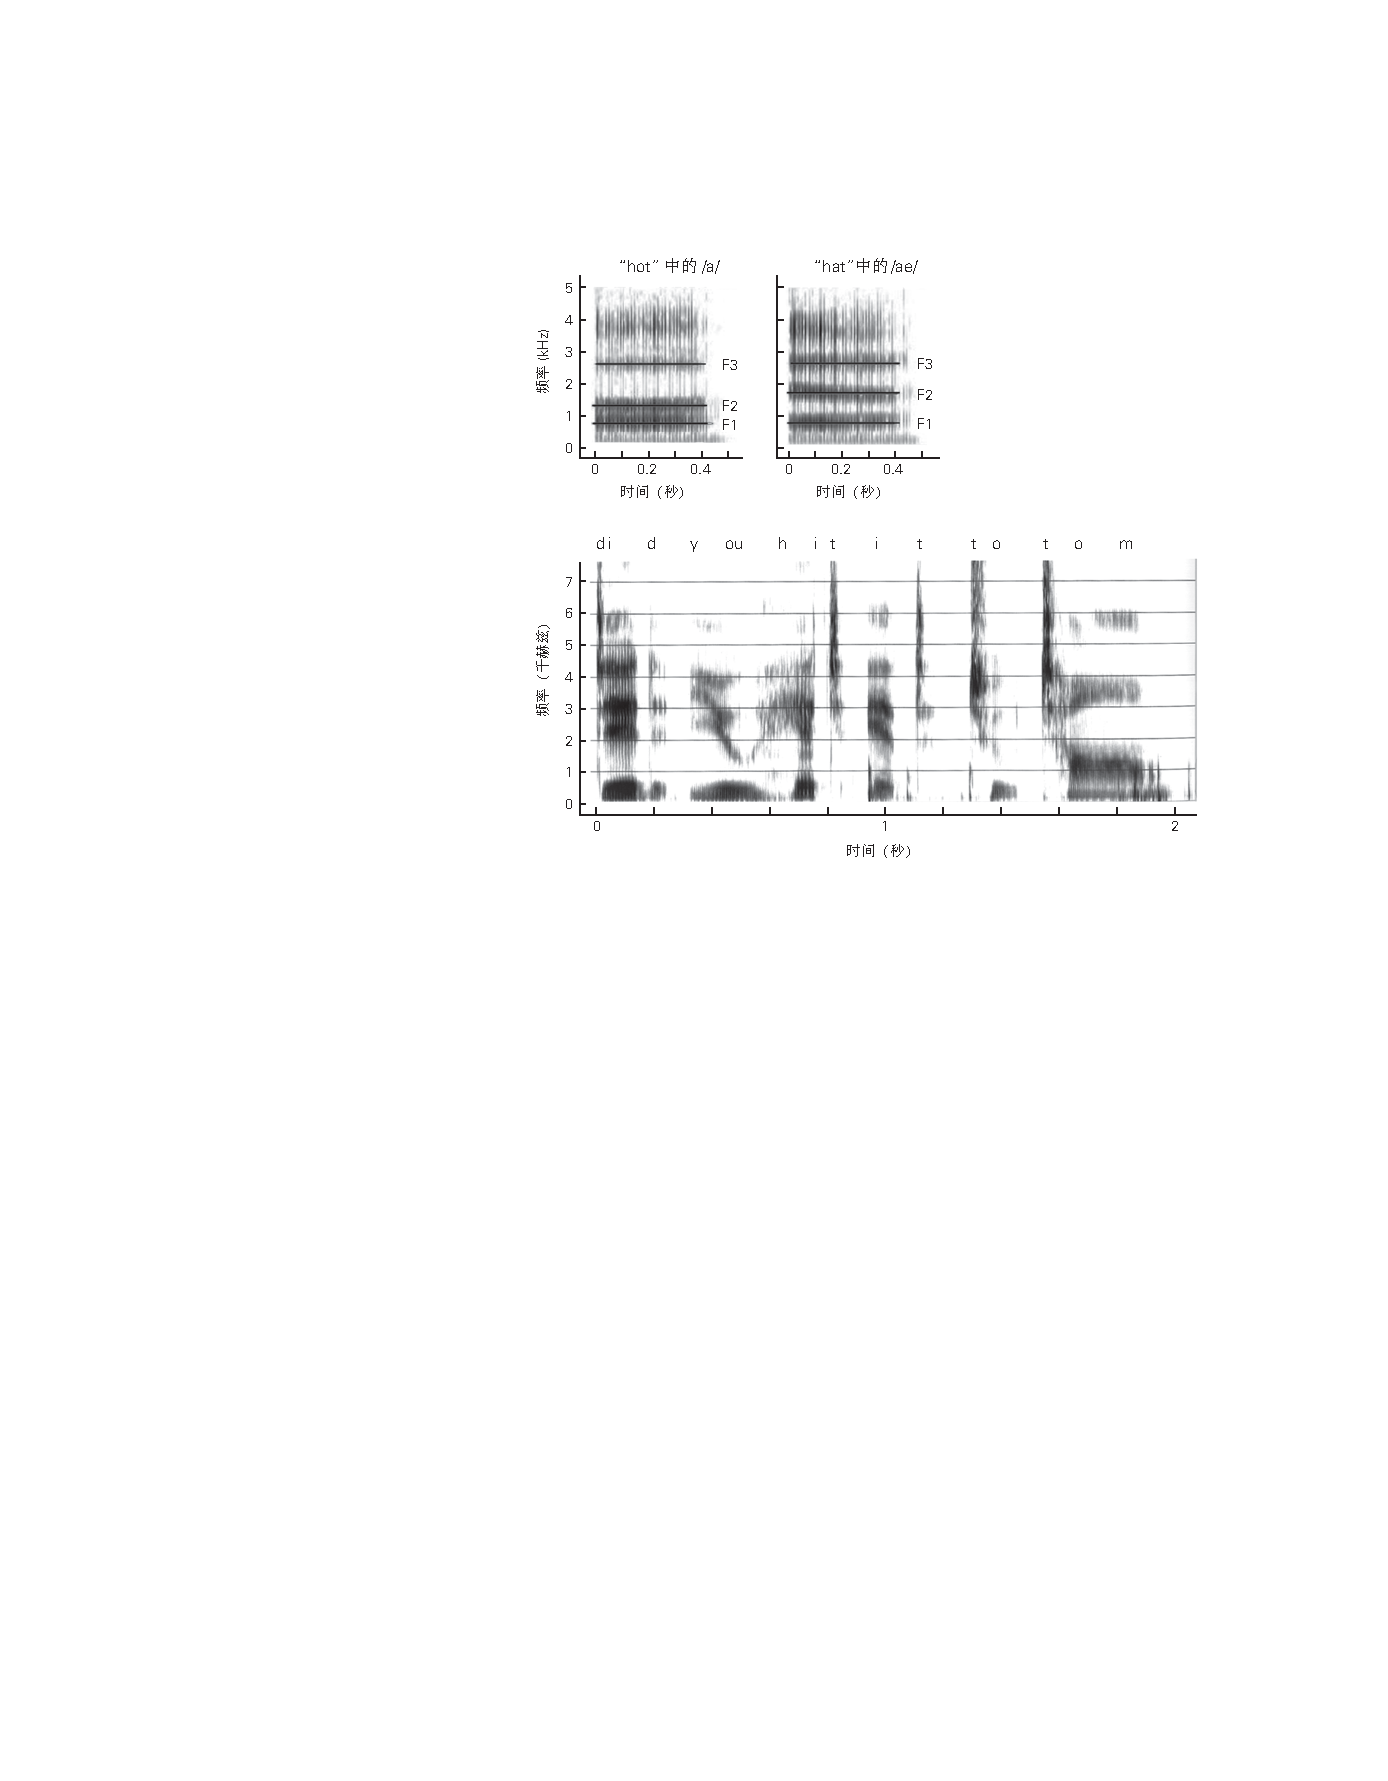
\includegraphics[width=0.81\linewidth]{chap55/fig_55_1}
	\caption{共振峰频率。
	共振峰是各种声音频率下能量集中的系统变化,代表声道的共振。
	它们在这里显示为语音频谱分析中时间的函数。
	两个单独说出的简单元音(/a/ 和 /ae/)的共振峰模式通过共振峰 2(F2)的差异来区分。
	“Did you hit it to Tom?”这句话的共振峰模式 说话缓慢而清晰地说明了正常说话背后的快速变化。}
	\label{fig:55_1}
\end{figure}


\textit{语音}规则规定了音素如何组合形成单词。
例如,英语和波兰语都使用音素 /z/ 和 /b/,但组合 /zb/ 在英语中是不允许的,而在波兰语中则很常见(如 \textit{Zbigniew} 这个名字)。


\textit{语素}是语言的最小结构单位,最好用前缀和后缀来说明。
例如,在英语中,前缀 \textit{un}(表示\textit{不})可以添加到许多形容词中以传达相反的含义(例如,\textit{不重要})。
后缀通常表示单词的时态或数量。
例如,在英语中,我们添加 \textit{s} 或 \textit{es} 来表示不止一个事物(\textit{bug} 变成 \textit{bugs},或者 \textit{box} 变成 \textit{boxes})。
为了表示一个规则动词的时态,我们给这个词加上一个词尾(例如,\textit{play} 可以变成 \textit{plays}、\textit{playing} 和 \textit{played})。
不规则动词不遵循规则(例如,\textit{go} 变成 \textit{went} 而不是 \textit{goed},\textit{break} 变成 \textit{broke} 而不是 breaked)。
每种语言都有一套不同的规则来改变单词的时态和数量。


最后,为了创造语言,单词必须串在一起。
\textit{语法}指定给定语言的单词和短语顺序。
例如,在英语中,句子通常符合主-动-宾顺序(例如,\textit{He eats cake}),而在日语中,它通常是主-宾-动词(例如,\textit{Karewa keeki o tabenzasu},字面意思是 \textit{He cake eats})。
语言在句子中较大元素(名词短语和动词短语)的顺序以及短语中单词的顺序方面存在系统差异,如英语和法语名词短语之间的差异所示。
在英语中,形容词在名词之前(例如,一个非常聪明的人),而在法语中,大多数形容词在名词之后(例如,\textit{un homme tres intelligent})。



\section{儿童的语言习得遵循通用模式}

无论文化如何,所有儿童最初都表现出通用的言语感知模式和产生模式,而这些模式并不取决于儿童听到的特定语言(图~\ref{fig:55_2})。
到第一年结束时,婴儿已经通过接触一种特定的语言学会了哪些语音单元在该语言中传达意义并识别可能的词,即使他们还不理解这些词。
到 12 个月大时,婴儿可以理解大约 50 个单词,并开始说出类似于母语的语言。
到 3 岁时,儿童会知道大约 1 千个单词(到成年时会达到 7 万个),会造出像成人一样的长句子,并且可以进行对话。
在 36 到 48 个月之间,孩子们以成人的方式对语法和非语法句子之间的差异做出反应,尽管使用最复杂的句子进行的测试表明,直到 7 到 10 岁的儿童后期才掌握语法的复杂性。


\begin{figure}[htbp]
	\centering
	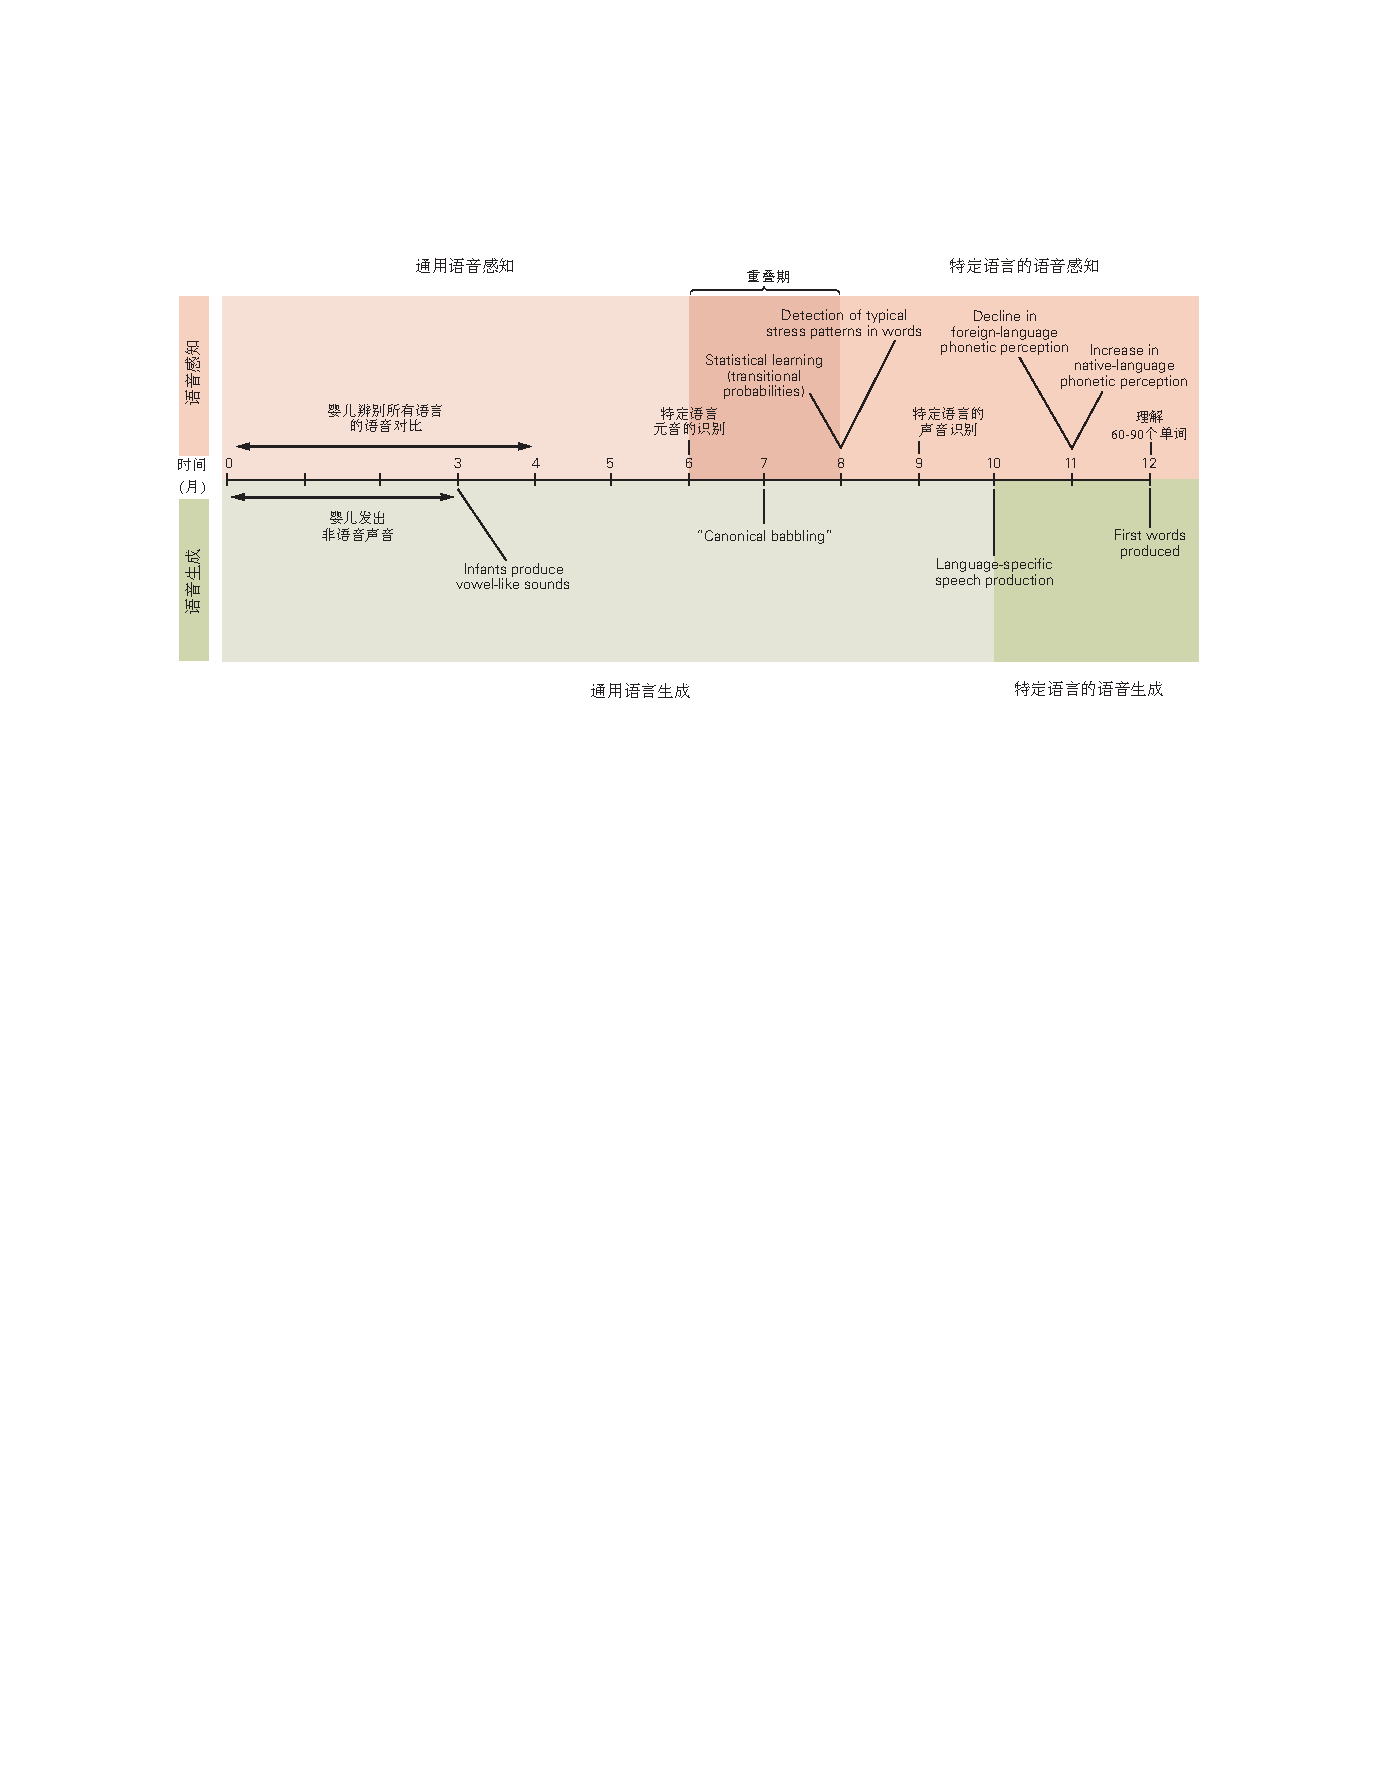
\includegraphics[width=1.0\linewidth]{chap55/fig_55_2}
	\caption{所有儿童的语言发展都按标准顺序进行。
		不同文化中儿童最初的语言感知和语言生成遵循语言通用模式。
		到生命的第一年结束时,特定语言的模式就会出现。
		在语音产生之前,语音感知变得特定于语言\cite{doupe1999birdsong}。
	}
	\label{fig:55_2}
\end{figure}


在 20 世纪下半叶,关于语言的本质和习得的辩论是由一位强大的学习理论家和一位强大的本土主义者之间的一次广为宣传的交流点燃的。
1957年,行为心理学家\textit{斯金纳}提出语言是通过学习获得的。
在他的《言语行为》一书中,斯金纳认为,语言与所有动物行为一样,是一种后天习得的行为,是儿童在外部强化和父母精心塑造的作用下发展起来的。
根据斯金纳的说法,婴儿学习语言就像老鼠学习按杆,通过监测和管理奖赏意外事件。
本土主义者\textit{诺姆$\cdot$乔姆斯基}撰写了一篇关于言语行为的评论,他持截然不同的立场。
乔姆斯基认为,传统的强化学习与人类习得语言的能力关系不大。
相反,他提出每个人都有一种与生俱来的“语言能力”,包括通用语法和通用语音;
接触一种特定的语言会触发一种语言的“选择”过程。


最近对婴儿和儿童语言习得的研究清楚地表明,婴儿期进行的学习类型与斯金纳所描述的依赖外部塑造和强化的学习方式不同。
与此同时,像乔姆斯基这样的先天论者的解释,婴儿听到的语言触发了几个先天选项中的一个的选择,也没有捕捉到这个过程。



\subsection{“普遍主义者”婴儿在 1 岁时变得语言专业化}

70 年代初期,心理学家\textit{彼得$\cdot$艾马斯}表明,婴儿特别擅长听觉区分世界语言语音单元的声学变化。
当语音以较小的相等步长在声学上发生变化以形成从一个语音单元到另一个语音单元的系列时,比如从 /ba/ 到 /pa/,\textit{艾马斯}表明婴儿可以辨别系列中位置的非常轻微的声学变化( “边界”),成年人听到两个语音类别之间的突然变化,这种现象称为分类感知。
\textit{艾马斯}证明,对于他们从未体验过的语言中的语音单元,婴儿可以在两个类别之间的语音边界处检测到这些轻微的声学变化,而成年人只有在他们能够流利使用的语言中检测到语音单元时才有这种能力。
例如,日本人发现很难听出美式英语 /r/ 和 /l/ 发音之间的声学差异。
两者都被认为是日语的 /r/,正如我们所见,说日语的人在造词时会互换使用这两种声音。


分类知觉最初被认为只存在于人类身上,但在 1975 年,认知神经科学家表明它存在于龙猫和猴子等非人类哺乳动物中。
从那时起,许多研究证实了这一结果(以及识别哺乳动物和鸟类之间的物种差异)。
这些研究表明,语音单元的演变受到先前存在的听觉结构和能力的强烈影响。
婴儿能够听到语音中所有可能的差异,这为他们学习任何语言做好了准备;
出生时,他们是语言学的“普遍主义者”。


言语产生与言语感知同时发展(图~\ref{fig:55_2})。
所有婴儿,无论文化如何,都会发出普遍的声音。
婴儿在 3 个月大时用类似元音的声音“咕咕”,在大约 7 个月大时用辅音-元音组合“牙牙学语”。
在第一年末,特定语言的言语产生模式开始出现在婴儿的自发话语中。
当孩子接近 2 岁时,他们开始模仿他们母语的声音模式。
中国幼儿的话语反映了普通话的音高、节奏和语音结构,而英国幼儿的话语听起来明显是英国式的。
早在 20 周大时,婴儿就会发展出模仿他们听到的其他人发出的声音的能力。
在发育的早期,婴儿就开始掌握产生“母语”所需的微妙运动模式。
在语言学习的早期阶段获得的言语运动模式会持续一生,并影响后来学习的第二语言的声音、节奏和节奏。


就在第一个单词出现之前,婴儿区分母语和非母语语音单元的能力发生了戏剧性的转变。
在 6 个月大时,婴儿可以辨别所有语言中使用的所有语音单元,但到 1 岁末,他们无法辨别 6 个月前成功识别的语音变化。
与此同时,婴儿明显更善于听取母语的语音差异。
例如,当美国和日本婴儿在 6 到 12 个月大时测试美式英语 /r/ 和 /l/ 的辨别力时,美国婴儿在 8 到 10 个月时明显改善,而日本婴儿下降,表明这 是语音学习的敏感期。
此外,婴儿在 7.5 个月大时的母语辨别能力预测了 14 到 30 个月大时已知单词、句子复杂性和平均话语长度的增长速度。


如果说一岁下半年是语言学习的敏感期,那么婴儿在这段时间接触一门新语言会发生什么?
他们学习吗?
当美国婴儿在 9 到 10 个月大时在实验室中接触普通话时,婴儿了解接触是否是通过与人的互动发生的;
通过电视或录音带接触到完全相同的材料而没有现场人际互动的婴儿不会学习(图~\ref{fig:55_3})。
在测试时,接触现场演讲者的小组的表现与在台湾长大并听了 10 个月普通话的婴儿的表现在统计上没有区别。 这些结果证实,在 9 个月大的时候,正确接触外语可以进行语音学习,支持这样的观点,即这是此类学习的敏感期。
然而,该研究还表明,社交互动在学习中发挥的作用比以前认为的更重要。


\begin{figure}[htbp]
	\centering
	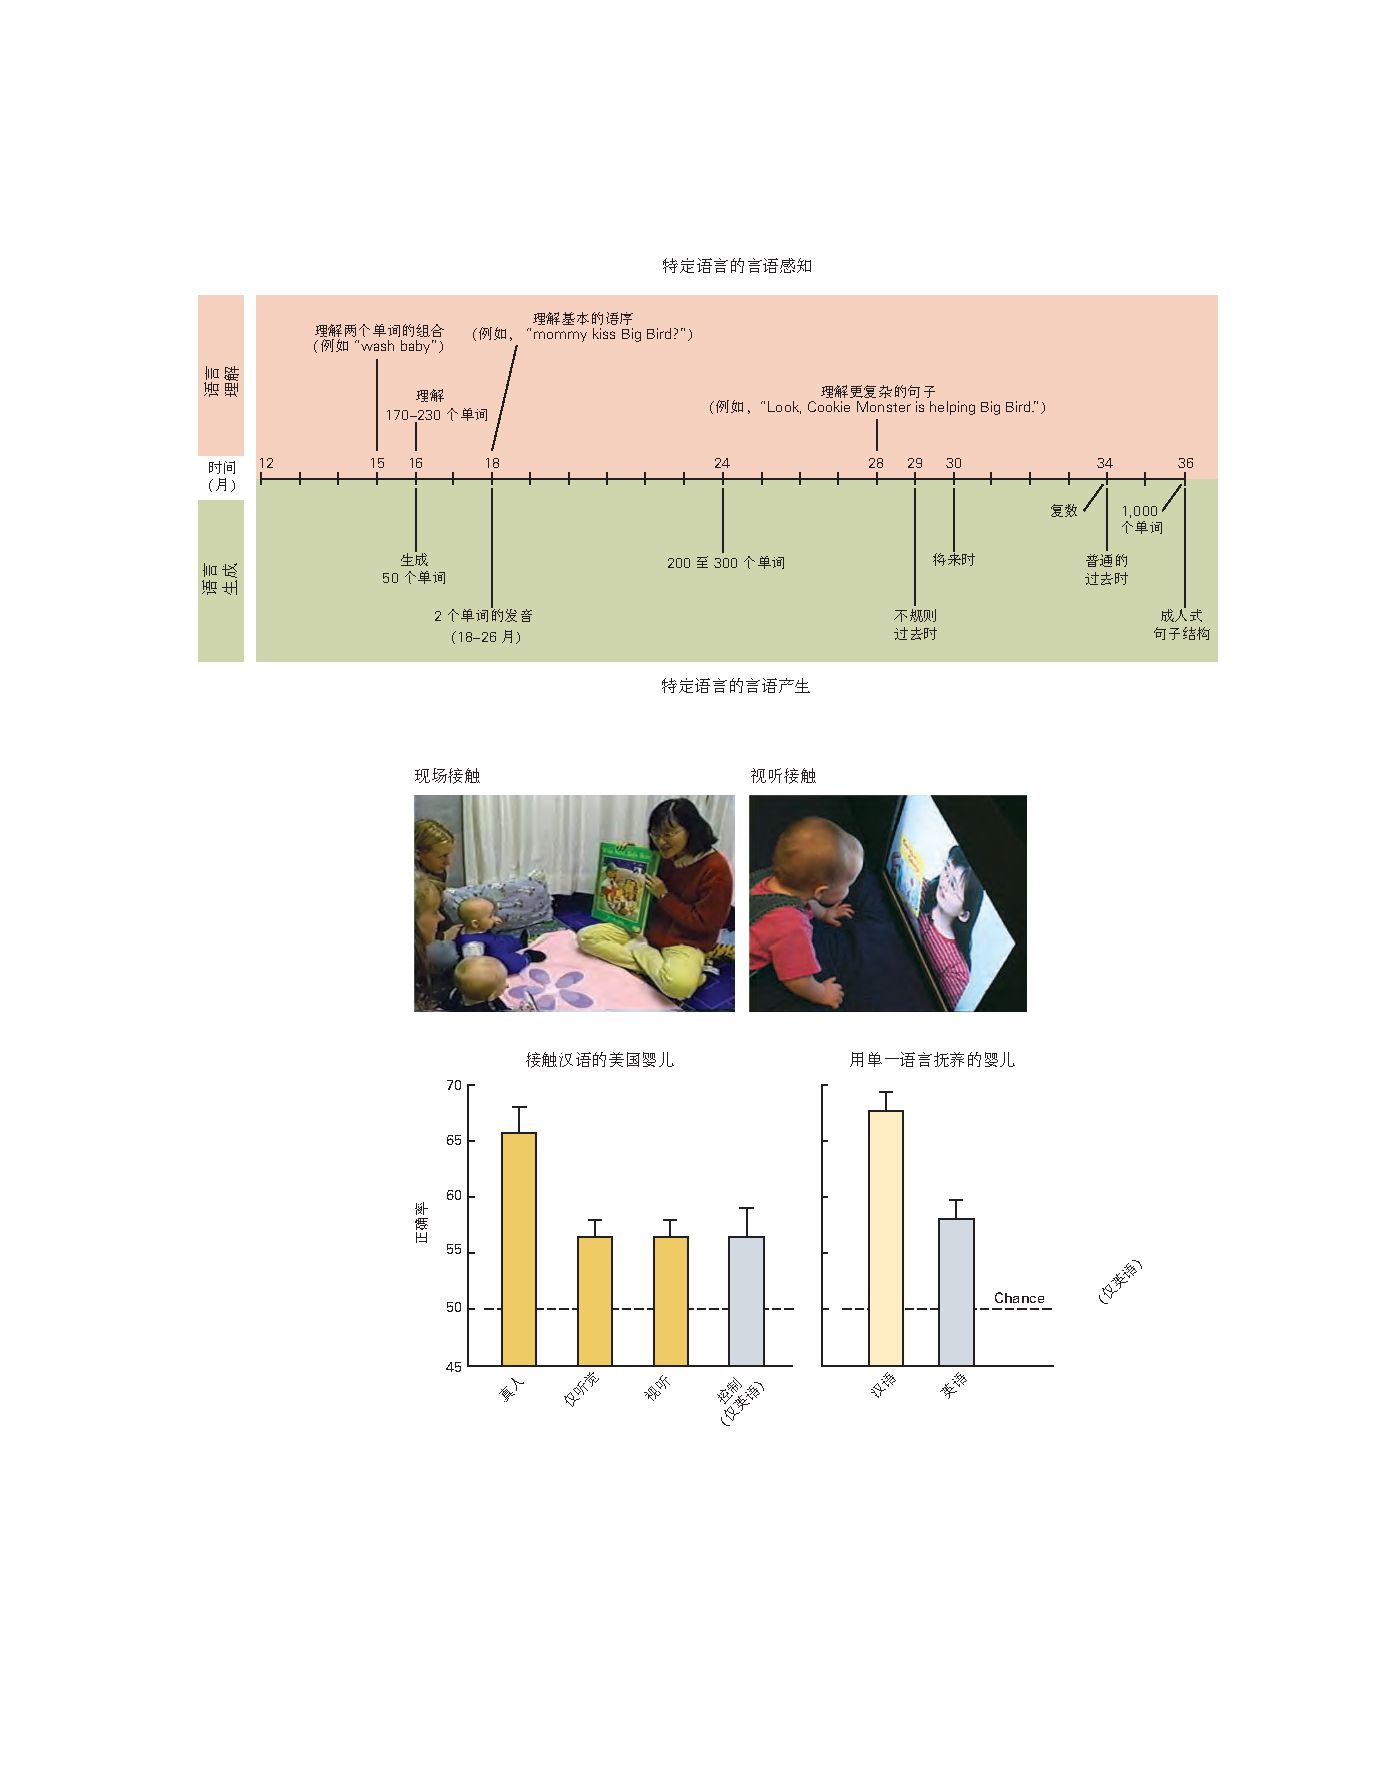
\includegraphics[width=1.0\linewidth]{chap55/fig_55_3}
	\caption{婴儿可以在 9 个月大时学习非母语的音素。
		三组美国婴儿在 9 至 10.5 个月大的 12 次 25 分钟课程中首次接触一种新语言(普通话)。
		一组与现场以普通话为母语的人互动;
		第二组通过电视接触到相同的材料;
		第三组只听录音。
		对照组有类似的语言课程,但只听到英语。
		接触后(11个月大),在所有组中测试了普通话音素的辨别能力\cite{kuhl2003foreign}。
		只有暴露在现场讲普通话的婴儿才能辨别普通话音素。
		通过电视或磁带接触的婴儿没有学习,他们的表现与对照婴儿(只听到英语)没有区别。
		美国婴儿接触现场讲普通话的表现与从出生就接触过普通话的同龄单语台湾婴儿的表现相当。}
	\label{fig:55_3}
\end{figure}


进一步的研究表明,婴儿跟踪导师眼球运动的程度(在她用外语命名物体时观察她正在看的东西)与接触新语言后语音和单词学习的神经测量密切相关,再次 在语言学习中涉及社会大脑区域。


婴儿获得社交线索的能力对语言学习至关重要,但在这个关键时期还有哪些其他技能可以促进学习?
研究表明,早期接触语音会引发内隐学习过程,该过程会增加对母语的辨别力,并降低婴儿天生的听觉区分所有其他语言语音单元的能力。
婴儿对他们听到的语言的统计特性很敏感。
声音的分布频率模式会影响婴儿 6 个月大时的语言学习。
婴儿开始根据语音原型将语音分类,这是他们语言中最常出现的语音单元。


美国和瑞典的 6 个月大的婴儿接受了英语和瑞典语原型元音测试,以检查婴儿是否能辨别元音的声学变化,就像不同说话者发出元音时发生的变化一样。
到 6 个月大时,美国和瑞典婴儿忽略了母语原型周围的声学变化,但没有忽略非母语原型。
\textit{保罗$\cdot$艾弗森}已经表明,语言体验会改变不同语言的说话者所关注的声学特征,并扭曲围绕类别原型的感知。
这使得刺激在感知上更类似于原型,这有助于解释为什么 11 个月大的日本婴儿在接触日语后无法区分英语 /r/ 和 /1/。



\subsection{视觉系统参与语言的产生和感知}

语言通常通过听觉-声音通道进行交流,但聋人通过视觉-手动通道进行交流。
自然手语,例如\textit{美国手语},是由聋人发明的,并且因国家/地区而异。
在发育过程中,聋哑婴儿用手“牙牙学语”的时间与听力正常的婴儿口牙牙牙牙语大致相同。
其他发育里程碑,例如第一个单词和两个单词的组合,也出现在听力正常婴儿的发育时间表上。


其他研究表明,另一种视觉信息,即谈话者的面部,不仅对交流非常有帮助,而且还会影响日常的言语感知。
我们都在嘈杂的聚会上体验过“唇读”的好处:观察说话者的嘴巴移动有助于我们在嘈杂的环境中理解讲话。
视觉在日常语音感知中发挥作用的最引人注目的实验室证明是当不一致的语音信息被发送到视觉和听觉模态时产生的错觉。
当受试者在观察一个人发出“ga”时听到音节“ba”时,他们报告说听到了中间发音“da”。
这些演示支持这样一种观点,即语音类别是通过听觉和视觉来定义的,并且感知是由视觉和声音共同决定的。



\subsection{韵律线索早在子宫内就已习得}

早在婴儿认识到世界上的事物和事件有名字之前,他们就记住了他们语言中典型的全球声音模式。
婴儿学习音高、持续时间和响度变化等韵律线索。
例如,在英语中,强/弱重音模式是典型的(如“BAby”、“MOMmy”、“TAble”和“BASEball”等词),而在某些语言中,弱/强模式占主导地位。
6 个月和 9 个月大的婴儿在英语或荷兰语单词之间进行听力选择时,在 9 个月大时(但 6 个月时不是)表现出对母语单词的听力偏好。


韵律线索可以传达语言信息(语言中语调和语调的差异,例如中文)和副语言信息,例如说话者的情绪状态。
即使在子宫内,胎儿也会通过聆听母亲的讲话来学习韵律线索。 某些声音通过骨传导传递到子宫;
这些通常是强烈的(高于 80 分贝)、低频声音(特别是低于 300 赫兹,但高达 1,000 赫兹并有一些衰减)。
因此,语音的韵律模式,包括特定语言和说话者的音高和重音和语调模式特征,被传递给胎儿,而传达语音单元和单词的声音模式被大大削弱。
出生时,婴儿表现出通过以下偏好学习了这种韵律信息:(1)母亲在怀孕期间所说的语言,(2)母亲的声音胜过另一位女性的声音,以及(3)阅读具有不同节奏和韵律的故事 在怀孕的最后 10 周内被母亲大声说出来。



\subsection{过渡概率有助于区分连续语音中的单词}

7 至 8 个月大的婴儿利用一个音节跟随另一个音节的概率来学习识别单词。
单词中音节之间的这种过渡概率很高,因为顺序保持固定。
例如,在单词 potato 中,音节“ta”总是跟在音节“po”之后(概率为 1.0)。
另一方面,单词之间,如字符串 hot potato 中的“hot”和“po”之间,转换概率要低得多。


心理学家\textit{珍妮$\cdot$扎弗兰}表明,婴儿将具有高过渡概率的语音单元和音节视为类词单位。
在一项实验中,婴儿听到 2 分钟的伪词串,例如 tibudo、pabiku、golatu 和 daropi,它们之间没有任何声音中断。
然后测试他们对这些伪词以及通过将一个词的最后一个音节与另一个词的两个初始音节组合而成的新词的识别(例如由 golatu 和 daropi 形成的 tudaro)。
婴儿识别出原始的伪词,但不能识别他们之前没有接触过的新组合,这表明他们使用过渡概率来识别单词。


这些学习形式显然不涉及斯金纳强化。
看护者不管理突发事件,而是通过加强婴儿进行的统计分析来逐渐塑造。
相反,婴儿的语言学习似乎也没有反映出根据语言经验选择先天提供的选项的过程。
相反,婴儿通过详细分析他们听到的自然语言中的统计变化模式以及对通过社交互动(例如,眼睛注视)提供的信息进行复杂分析来学习语言。
学习这些模式反过来会改变感知以支持母语。
总之,语言的统计特性和语言交互过程中提供的社交线索都有助于婴儿学习。
语言进化为利用婴儿天生能够识别的各种线索。
这反映了这样的论点,即语音单元的发展受到哺乳动物听觉特征的显著影响,确保婴儿会发现很容易区分音素,即语言中意义的基本单位。



\subsection{语言学习有关键期}

儿童比成人更自然、更有效地学习语言,鉴于成人的认知技能更优越,这是一个悖论。
为什么会这样?


许多人认为语言习得是在发展的关键时期学得最好的技能的一个例子。
\textit{埃里克$\cdot$勒纳伯格}提出,青春期的成熟因素会导致控制语言习得的神经机制发生变化。
支持这一观点的证据来自对 3 至 39 岁期间沉浸在英语环境中的美国中国和韩国移民的经典研究。
当被要求识别包含语法错误的句子中的错误时,这对母语人士来说是一项简单的任务,第二语言学习者的回答随着到达美国的年龄而下降。
当比较从出生开始接触\textit{美国手语}的个体与 5 至 12 岁接触\textit{美国手语}的个体时,会出现类似的趋势。
出生时接触过的人最擅长识别\textit{美国手语}错误,5 岁时接触过的人稍差,12 岁以后接触过的人差得多。


是什么限制了我们在青春期后学习一门新语言的能力?
发展研究表明,先前的学习起着一定的作用。
学习母语会产生检测该语言声学模式的神经承诺,而这种承诺会干扰以后学习第二语言。
早期接触语言会导致神经回路“调整”以检测该语言的语音单元和韵律模式。
对母语的神经承诺增强了检测基于已经学习的模式的能力(例如,语音学习支持单词学习),但降低了检测不符合模式的能力。
学习说一种语言所需的运动模式也会导致神经承诺。
为一种语言学习的运动模式(例如,法语中的嘴唇变圆)可能会干扰第二语言(例如,英语)发音所需的运动模式,因此可能会阻碍在没有口音的情况下发音第二语言的努力。
在生命的早期,可以很容易地学习两种或多种语言,因为在神经模式完全建立之前,干扰影响很小。


神经生物学家\textit{高雄$\cdot$亨施}一直致力于确定开启和关闭神经发育关键学习期的化学开关,包括动物和人类的开关。
\textit{亨施}发现,神经递质\textit{$\gamma$-氨基丁酸}通过抑制兴奋性神经元的放电来开启关键期,使它们与抑制性神经元的放电达到平衡,从而形成\textit{兴奋-抑制}平衡。
很难在人类中验证这一假设的研究,但对通过服用精神药物(\textit{5-羟色胺再吸收抑制剂})治疗抑郁症而改变胎儿\textit{兴奋-抑制}平衡的母亲的婴儿进行的调查支持\textit{兴奋-抑制}假设。
氟西汀的脱靶效应之一是增加某些\textit{$\gamma$-氨基丁酸}受体对\textit{$\gamma$-氨基丁酸}的敏感性。
与产前未暴露于\textit{5-羟色胺再吸收抑制剂}的抑郁母亲的婴儿和未患抑郁症或\textit{5-羟色胺再吸收抑制剂}的对照母亲的婴儿相比,产前暴露于\textit{5-羟色胺再吸收抑制剂}的婴儿表现出加速的语音学习过程,表明婴儿语音感知早期转变的确定时间可以改变。


我们不会在以后的生活中完全失去学习一门新语言的能力,但要困难得多。
无论学习开始的年龄如何,第二语言学习都可以通过模仿早期学习关键组成部分的训练方案得到改善,在社交环境中长时间聆听(沉浸),同时使用听觉和视觉信息,以及接触简化的环境 和类似“父母语”的夸张言论。



\subsection{“父母语”说话风格增强语言学习}

每个人都同意,当大人和他们的孩子说话时,他们听起来很不寻常。
1960年代初期,语言学家和人类学家在聆听世界各地的语言时发现,“妈妈语”(或“父母语”,父亲也会这样说)是一种特殊的说话方式,用于称呼婴幼儿。
\textit{父母语}音调较高,速度较慢,语调轮廓夸张,易于识别。
与针对成人的语音相比,男性和女性的声音音调平均提高了一个八度。
语音单元被说得更清楚并且在声学上被夸大了,从而增加了语音单元的声学独特性。
成人对婴儿说话只是夸大了那些对他们的母语至关重要的语言特征。
例如,在与婴儿交谈时,中国母亲会夸大普通话中对词义至关重要的四个声调。


当给予选择时,婴儿更喜欢听婴儿指导的而不是成人指导的讲话。
当婴儿被允许通过向左或向右转动头部来激活婴儿定向或成人定向语音的录音时,他们将转向需要打开婴儿定向语音的任何方向。


心理学家\textit{奈兰$\cdot$·拉米雷斯-埃斯帕扎}和\textit{阿德里安$\cdot$·加西亚-塞拉}最近的研究表明,11 个月和 14 个月大的婴儿在家中使用父母语的程度与 24 个月大时孩子的语言发展密切相关,并且在 36 个月大时仍保持强相关。
这种关系适用于单语和双语儿童。
然而,在双语儿童中,两种语言的早期进步因父母所说的语言而异。
例如,西班牙语父母语会增强孩子对西班牙语而非英语的行为和神经反应,反之亦然。
在语言接触量和父母语使用率低的家庭中长大的孩子在进入学校时往往会表现出语言和识字方面的缺陷,而这些缺陷与大脑中与语言相关的区域的功能激活减少有关。



\subsection{成功的双语学习取决于学习第二语言的年龄}

大脑如何处理两种语言?
行为数据表明,如果从出生时就开始接触两种语言,那么儿童会在与单语同龄人相同的年龄达到语言的里程碑,他们会在单语儿童的基准年龄咕咕叫、喋喋不休并说出单词。
双语经历会产生“混淆”的观点已被测量“概念”词汇的研究所揭穿,即无论孩子使用何种语言表达该知识的单词知识。
较早的研究仅用婴儿两种语言中的一种来测量单词,与单语者相比,这种单词计数通常显示词汇量减少。
概念词汇分数表明,双语儿童的词汇量达到或超过单语儿童的词汇量。


青春期后接触第二语言表明学习新语言的程度有限。
无论是语音规则、词尾还是句法测试,7 岁后学习一门新语言的能力似乎每 2 年下降一次,这表明青春期后习得第二语言相当困难。


双语婴儿的大脑测量反映了这些行为数据。
心理学家\textit{纳亚$\cdot$费金$\cdot$拉米雷斯}使用\textit{脑磁图}表明,从出生开始就接触两种语言(英语和西班牙语)的 11 个月大婴儿的颞上区激活对于两种语言的声音是相同的,并且大脑对英语声音的反应是相当于同龄的英语单语婴儿。
与单语婴儿相比,双语婴儿在听语音时的前额叶皮层也表现出更大的激活,前额叶皮层是一个调解注意力的区域;
这一发现与双语儿童(以及成人)表现出与注意力相关的卓越认知技能的事实是一致的。
可以说,聆听两种语言需要多次转移注意力才能激活一种语言而不是另一种语言。


如果第二语言是在发育后期获得的,那么接触的年龄和最终的熟练程度会影响大脑处理这两种语言的方式。
在“晚期”双语者(青春期后学习第二语言的人)中,第二语言和母语在对语言敏感的左额叶区域的空间分离区域中进行处理。
在“早期”双语者(那些在儿童时期就掌握了两种语言的人)中,两种语言在同一个左额叶区域进行处理。



\section{一种新的语言神经基础模型已经出现}

\subsection{许多专门的皮层区域有助于语言处理}

% https://picture.iczhiku.com/weixin/message1625543107586.html
经典的\textit{韦尼克-格施温德}语言神经模型基于布洛卡\cite{broca1861remarques}、韦尼克\cite{wernicke1974aphasische}、利什特海姆\cite{lichtheim1885aphasia} 和格施温德\cite{geschwind1970organization}的工作。
% 利什特海姆氏征(皮质性失语患者不能言语,但能用指示意) 
在韦尼克-格施温德模型中,口语中包含的声学线索在听觉通路中被处理并传递到韦尼克区,在那里单词的含义被传递到更高的大脑结构。
弓状束被认为是一种单向通路,可将信息从韦尼克区带到布罗卡区,从而实现语音生成。
韦尼克区和布罗卡区都与关联区相互作用。
韦尼克-格施温德模型构成了临床神经学家今天仍在使用的失语症实用分类的基础(表~\ref{tab:55_1})。


\begin{table}[htbp]
	\caption{失语症主要类型的鉴别诊断} \label{tab:55_1} \centering
	\begin{tabular}{llllll}
		\toprule
		失语症类型 & 说话方式 & 理解 & 重复能力 & 其他标志 & 影响的区域 \\
		\midrule
		布洛卡 & \makecell[l]{不流利、\\需要努力的} & \makecell[l]{基本上保留了\\单个单词和语\\法简单的句子} & 受损 & \makecell[l]{右偏瘫\\(手臂>腿部);\\患者意识到\\缺陷,可能\\会抑郁} & \makecell[l]{左后额叶皮层\\和底层结构} \\
		韦尼克 & \makecell[l]{流利、丰富、\\表达清晰、\\旋律优美} & 受损 & 受损 & \makecell[l]{无运动标志;\\患者可能\\焦虑、烦躁、\\兴奋或偏执} & \makecell[l]{左后颞\\中上皮层} \\
		传导 & \makecell[l]{流利,有一些\\发音缺陷} & 完整或大部分保存 & 受损 & \makecell[l]{通常没有;患者\\右臂可能有皮层\\感觉丧失或无力} & \makecell[l]{左颞上回\\和边缘上回} \\
		全局 & \makecell[l]{缺乏、不流利} & 受损 & 受损 & \makecell[l]{右侧偏瘫} & \makecell[l]{左侧外侧裂\\巨大病变} \\
		皮层运动性 & \makecell[l]{非流利、\\轰响的} & 完整或大部分保存 & 完整或大部分保存 & \makecell[l]{有时是\\右侧无力} & \makecell[l]{布罗卡区前方\\或上方变} \\
		经皮层感觉 & \makecell[l]{流利,缺乏} & 受损 & 完整或大部分保存 & \makecell[l]{无运动标志} & \makecell[l]{韦尼克区后\\方或下方} \\
		\bottomrule
	\end{tabular}
\end{table}


基础和临床神经科学的进步、更复杂的功能性大脑成像工具的出现、结构性大脑成像的先进方法以及越来越多的结合大脑和行为测量的研究导致了新的“双流”模型的发展。
在双流模型中,语言处理被认为涉及由不同大脑区域组成的大规模网络,每个区域都有专门的功能,以及连接它们的白质束。


这种语言处理的双流模型类似于视觉系统中公认的“内容”和“空间”双流模型。
听觉信息处理的两个皮层流的存在首先由\textit{约瑟夫$\cdot$罗斯柴可}提出。
\textit{格雷戈里$\cdot$希科克}和\textit{大卫$\cdot$波佩尔}进一步阐述了双流模型,此后\textit{安吉拉$\cdot$弗里德里希}以及其他研究语言神经生物学的人进一步扩展了该模型。
图~\ref{fig:55_4}~显示了双流模型的基本组件。


\begin{figure}[htbp]
	\centering
	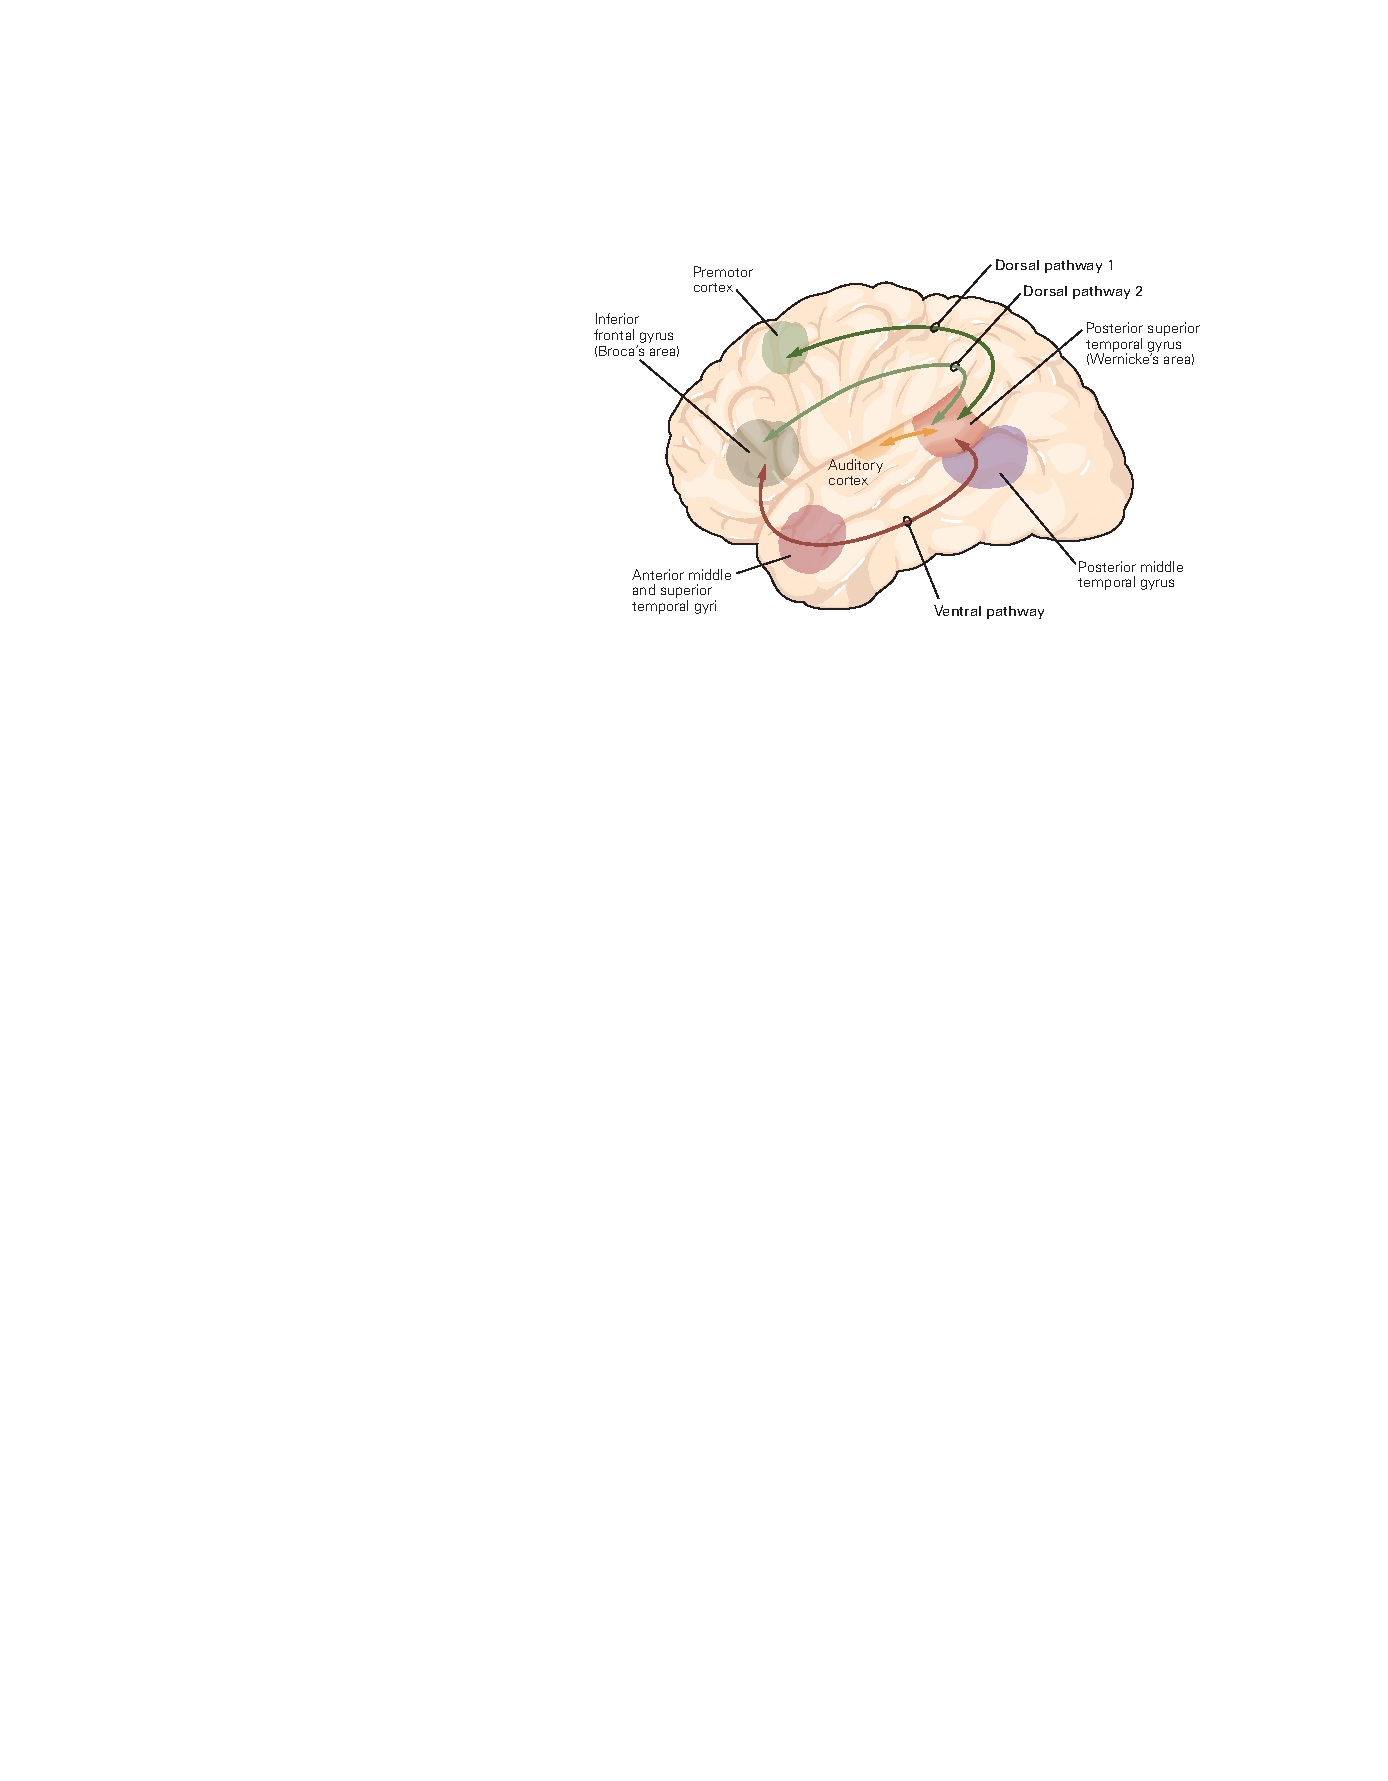
\includegraphics[width=0.77\linewidth]{chap55/fig_55_4}
	\caption{语言处理的双流模型。
		语音信号的\textit{时间}分析和\textit{频谱}分析发生在\textit{听觉皮层}的双侧,然后在\textit{颞上回后部}进行语音分析(黄色箭头)。
		然后,处理过程分为两条独立的途径:
		将语音映射到\textit{运动}程序的背侧流和将语音映射到\textit{意义}的腹侧流。
		背侧通路以左半球为主,其节段延伸至\textit{前运动皮层}(背侧通路1)和\textit{额下回}(背侧通路2)。
		腹侧通路发生在双侧,并延伸到前颞叶和后下额\cite{hickok2007cortical,skeide2016ontogeny}。}
	\label{fig:55_4}
\end{figure}


与经典的\textit{韦尼克$\cdot$格施温德模型}相比,双流模型包含更多的皮层区域,这些区域在大脑中分布更广泛,并在专门的大脑区域之间添加了关键的连接双向通路。
语言处理模型的这些改进归功于结构性脑成像技术的进步,例如\textit{弥散张量成像}和弥散加权成像,这些技术提供了连接各个皮层区域束中白质的微观尺度的定量测量,并允许整个大脑神经束的详细描绘(纤维束成像)。


在双流模型中,听觉语音的初始光谱时间处理是在听觉皮层中双侧进行的。
然后,该信息被双侧传送到\textit{颞上回后部},在那里发生语音级处理。
语言处理然后分化为背侧“感觉运动流”,将声音映射到发音,以及腹侧“感觉-概念”流,将声音映射到意义。


双向背侧流将听觉语言信息与产生语言的运动计划联系起来。
背侧流在侧脑室上方通过,将声音映射到发音表征上,将下额叶、运动前皮层和脑岛(所有这些都参与发音发音)连接到通常被认为是韦尼克区的区域。
它被认为包括两条通路:
\textit{背侧通路 1} 将\textit{颞上回后部}连接到\textit{前运动皮层},
\textit{背侧通路 2} 将\textit{颞上回后部}连接到\textit{布罗卡区}。
\textit{背侧通路 2} 涉及对语音的高阶分析,例如基于语法和使用更复杂概念的解释语言来区分含义的细微差异。
背侧流是强烈的左半球优势。
\textit{弓状束}和\textit{上纵束}是白质纤维束,介导背侧流的通讯。


腹侧流通过\textit{外侧裂}下方,由\textit{上颞叶}和\textit{中颞叶}区域以及后下额叶区域组成。
该流传递用于听觉理解的信息,这需要将听觉信号转换为心理词典中的表示,心理词典是一种将单个单词形式与其语义联系起来的“基于大脑的词典”。
该流包括下额枕束、钩束和末端纤维囊系统,并且主要是双侧的。


双流模型中包含的大脑皮层区域还与大脑两个半球的空间分布区域相互作用,这些区域提供对语言处理至关重要的额外信息。
这些区域包括前额叶皮层和扣带皮层,它们分别发挥执行控制和调节注意力过程,以及内侧颞叶、额叶和顶叶区域中涉及记忆检索的区域。




\subsection{语言的神经结构在婴儿期迅速发展}

婴儿期语言发展的研究需要一种方法来记录行为的显著变化,并将这些变化与大脑功能和形态随时间的变化联系起来。
在过去十年中,婴儿大脑的神经影像学方法有了很大改进,可以详细评估语言网络所需的特殊区域和结构连接的发展进程。
例如,发育神经科学家已经为 3 个月和 6 个月大的婴儿大脑创建了普通婴儿大脑模型和大脑图谱。
这些模型表明,对成年语言处理至关重要的大脑结构,如下额叶皮层、运动前皮层和颞上回,支持婴儿早期的语言处理。
使用\textit{弥散张量成像}和肌束成像的研究表明,弓状束和钩状束在 3 个月大时连接语言区域。


\textit{丹妮拉$\cdot$佩拉尼}使用\textit{功能性磁共振成像}和\textit{弥散张量成像}深入研究了 1 至 3 日龄婴儿语言神经基础的发育。
\textit{佩拉尼}的\textit{功能性磁共振成像}研究表明,听语音会激活婴儿双侧颞上回,并且在左半球,这种激活会延伸到颞叶、额下回和顶叶下部。
\textit{佩拉尼}对同一名新生儿的\textit{弥散张量成像}研究表明,大脑半球内的联系较弱,但半球之间的联系很强。
尽管如此,通过极端纤维囊系统将额下回腹侧部分连接到颞叶皮层的腹侧纤维束在新生儿和两个半球中都很明显。
连接颞叶皮层和前运动皮层的背侧通路也存在于新生儿身上,尽管在成人中连接颞叶皮层和布罗卡区的背侧通路在新生儿中检测不到。
感觉区域和前运动皮层之间的这些早期连接很重要,因为它们可能允许感觉到运动的映射,这对于早期模仿语言的声音和单词的发展至关重要。


\textit{延斯$\cdot$布劳尔}及其同事重复了这些关于新生儿腹侧和背侧通路发育的发现,揭示了连接颞区和额下回的腹侧连接在成熟过程中的首要地位。
\textit{布劳尔}还证实了背侧通路在出生时连接了颞叶和前运动皮层,并表明通往下额回的背侧通路后来发育。
布劳尔对 7 岁的儿童和成人使用了相同的方案。
在 7 岁儿童中,背侧通路完全连接听觉区和额下回,但在成人中,它具有更广泛和深远的联系。


对早在 2 个月大的婴儿进行的\textit{脑电图}和\textit{脑磁图}功能性脑成像研究表明,涉及经典和现代语言处理模型的下额叶和颞叶皮层被语音(音节、单词和句子)双侧激活。
这一发现支持左半球专业化随着时间的推移而增加的假设,在第一年末音节显示出主要的左半球专业化,到 2 岁时单词和儿童中期的句子。


对小婴儿的\textit{脑电图}和\textit{脑磁图}研究表明,婴儿被动地听母语和非母语音节,其结果与本章前面描述的行为转变一致。
几个婴儿实验室已经表明,在发育早期测量的大脑对语言的反应活动提供了预测几年后语言技能的敏感标记。
这些研究有望最终确定婴儿的大脑测量值,这些测量值表明涉及语言的发育障碍风险,例如孤独症谱系障碍、阅读障碍和特定语言障碍。
及早识别可以更早、更有效地干预这些障碍,改善这些儿童及其家庭的结果。


使用功能性\textit{脑磁图}脑成像的婴儿研究表明,在 7 个月大时,母语和非母语语音音节不仅激活婴儿大脑的上颞区,还激活额叶下区和小脑,从而在他们听到的语音模式和他们听到的语音之间建立联系 他们用来喋喋不休和模仿的运动计划。
到 12 个月大时,语言体验会改变大脑感觉和运动区域的激活模式。


母语声音的听觉激活变得更强,表明大脑区域已经开始专门处理母语语音。
相比之下,布罗卡区和小脑的运动激活都会随着非本地声音的反应而增加,因为到 12 个月时,婴儿已经具备足够的感觉运动知识来模仿本地声音和一些单词,并且已经将存储的听觉模式(如“杯子”和“球”)到生产它们所必需的运动计划。
但他们无法对外语声音和单词进行感觉运动联想,因为无法生成必要的运动计划。
因此,当婴儿努力为他们从未经历过的声音或单词制定运动计划时,我们会看到更长、更分散的激活。
对 7 个月大的婴儿进行的基于全脑体素的纵向形态测量学研究也显示了运动学习在语言发展中的重要性,该研究表明小脑中的灰质浓度与这些婴儿在 1 岁时可以产生的单词数量相关 年龄。


在接下来的 5 年里,专注于语言网络发展的大脑研究可能会出现爆炸式增长。
在许多实验室中,这些大脑测量将与行为测量相关联,从而能够创建描述语言体验如何改变婴儿大脑以增加其对儿童所接触的一种或多种语言的专业化的模型。
成人语言网络中已知的经典大脑区域(特别是左右颞叶皮层和左下额叶皮层),在出生时就已经被语言激活的发现让人想起乔姆斯基对先天语言能力的看法。



\subsection{左半球主导语言}

目前的语言处理观点认为,虽然将语音转化为意义所必需的神经回路可能存在于两个半球,但左半球更专门用于语言处理。
这种左半球优势随着成熟和学习而发展。


来自各种来源的证据表明,左半球的语言专业化在婴儿期发展迅速。
单词学习就是一个很好的例子。
\textit{黛博拉$\cdot$米尔斯}和她的同事们使用事件相关电位来追踪神经信号的发展,这些神经信号是针对儿童所知道的单词而产生的。
她的研究表明,年龄和语言能力都会导致对已知单词的神经反应强度发生变化,以及 13 至 20 个月大时半球优势的变化。
在研究的最早年龄段,已知单词会激活大脑中广泛且双向分布的模式。
随着婴儿接近 20 个月和词汇量的增长,激活模式转变为在颞叶和顶叶区域以左半球为主。
在说话晚的人中,这种转变被推迟到将近 30 个月。
在 24 个月大的孤独症儿童中,这种左半球优势的明显程度预示着儿童在 6 岁时的语言、认知和适应能力。


几项研究表明,成年后沉浸在第二语言中会导致上纵束生长,这是一种对语言很重要的白质纤维束。
神经科学家\textit{平$\cdot$玛米亚}与遗传学家\textit{埃文$\cdot$艾克勒}合作,使用\textit{弥散张量成像}证明,中国大学生右半球上纵束的白质完整性随着他们在英语浸入式课程中度过的天数成比例增加,而在学习后减少沉浸结束。
此外,对\textit{儿茶酚氧位甲基转移酶}基因多态性的分析显示了对这种关系的影响,具有两个变体的学生表现出这些变化,而具有第三个变体的学生的白质特性没有随语言经验发生变化。


人们对调查语言背后的大脑机制的选择性的大脑研究非常感兴趣。
神经科学家\textit{南希$\cdot$坎韦施}对视觉系统的研究表明,某些视觉区域(梭形面部区域)对特定刺激具有高度选择性,例如面部。
对于语音分析的大脑区域也提出了类似的主张。
例如,\textit{坎韦施}的小组提出布罗卡区包含许多子区域,每个子区域都对特定语言水平具有高度选择性。
关于选择性的其他研究,特别是在开发过程中,将是未来研究的重点。


\textit{海伦$\cdot$内维尔}和\textit{劳拉$\cdot$安妮$\cdot$佩蒂托特}表明,左半球不仅会被听觉刺激激活,还会被具有语言意义的视觉刺激激活。
聋人在左半球语音处理区域处理手语。
这些研究表明,语言网络处理语言信息时不考虑模态。



\subsection{韵律根据传达的信息同时影响右半球和左半球}

语言中的韵律线索可以是语言性的,传达语义,就像普通话或泰语中的声调一样,也可以是副语言性的,表达我们的态度和情感。
声音的音高携带着两种信息,而大脑对每种信息的处理也不同。


音高的情绪变化涉及右半球,主要是右额叶和颞叶区域。
情感信息有助于传达说话者的心情和意图,这有助于解释句子的意思。
右半球受损的患者说话时常常带有不适当的重音、时机和语调,而且他们的讲话听起来情绪低落;
他们也经常无法理解他人言语中的情感暗示。


正如神经影像学研究所证明的那样,音高的语义变化涉及不同的大脑活动模式。
\textit{杰克逊$\cdot$格兰登}使用了一种新颖的实验设计,使用带有中国本土音调或非泰国本土音调的中文音节。
汉语和泰语使用者的\textit{功能性磁共振成像}结果显示,与非母语相比,带有母语的音节在左侧颞叶平面的激活更高(图~\ref{fig:55_5})。
右半球没有表现出这种双重分离,支持这样一种观点,即语言处理发生在左半球,即使对于通常在右半球处理的听觉信号也是如此。


\begin{figure}[htbp]
	\centering
	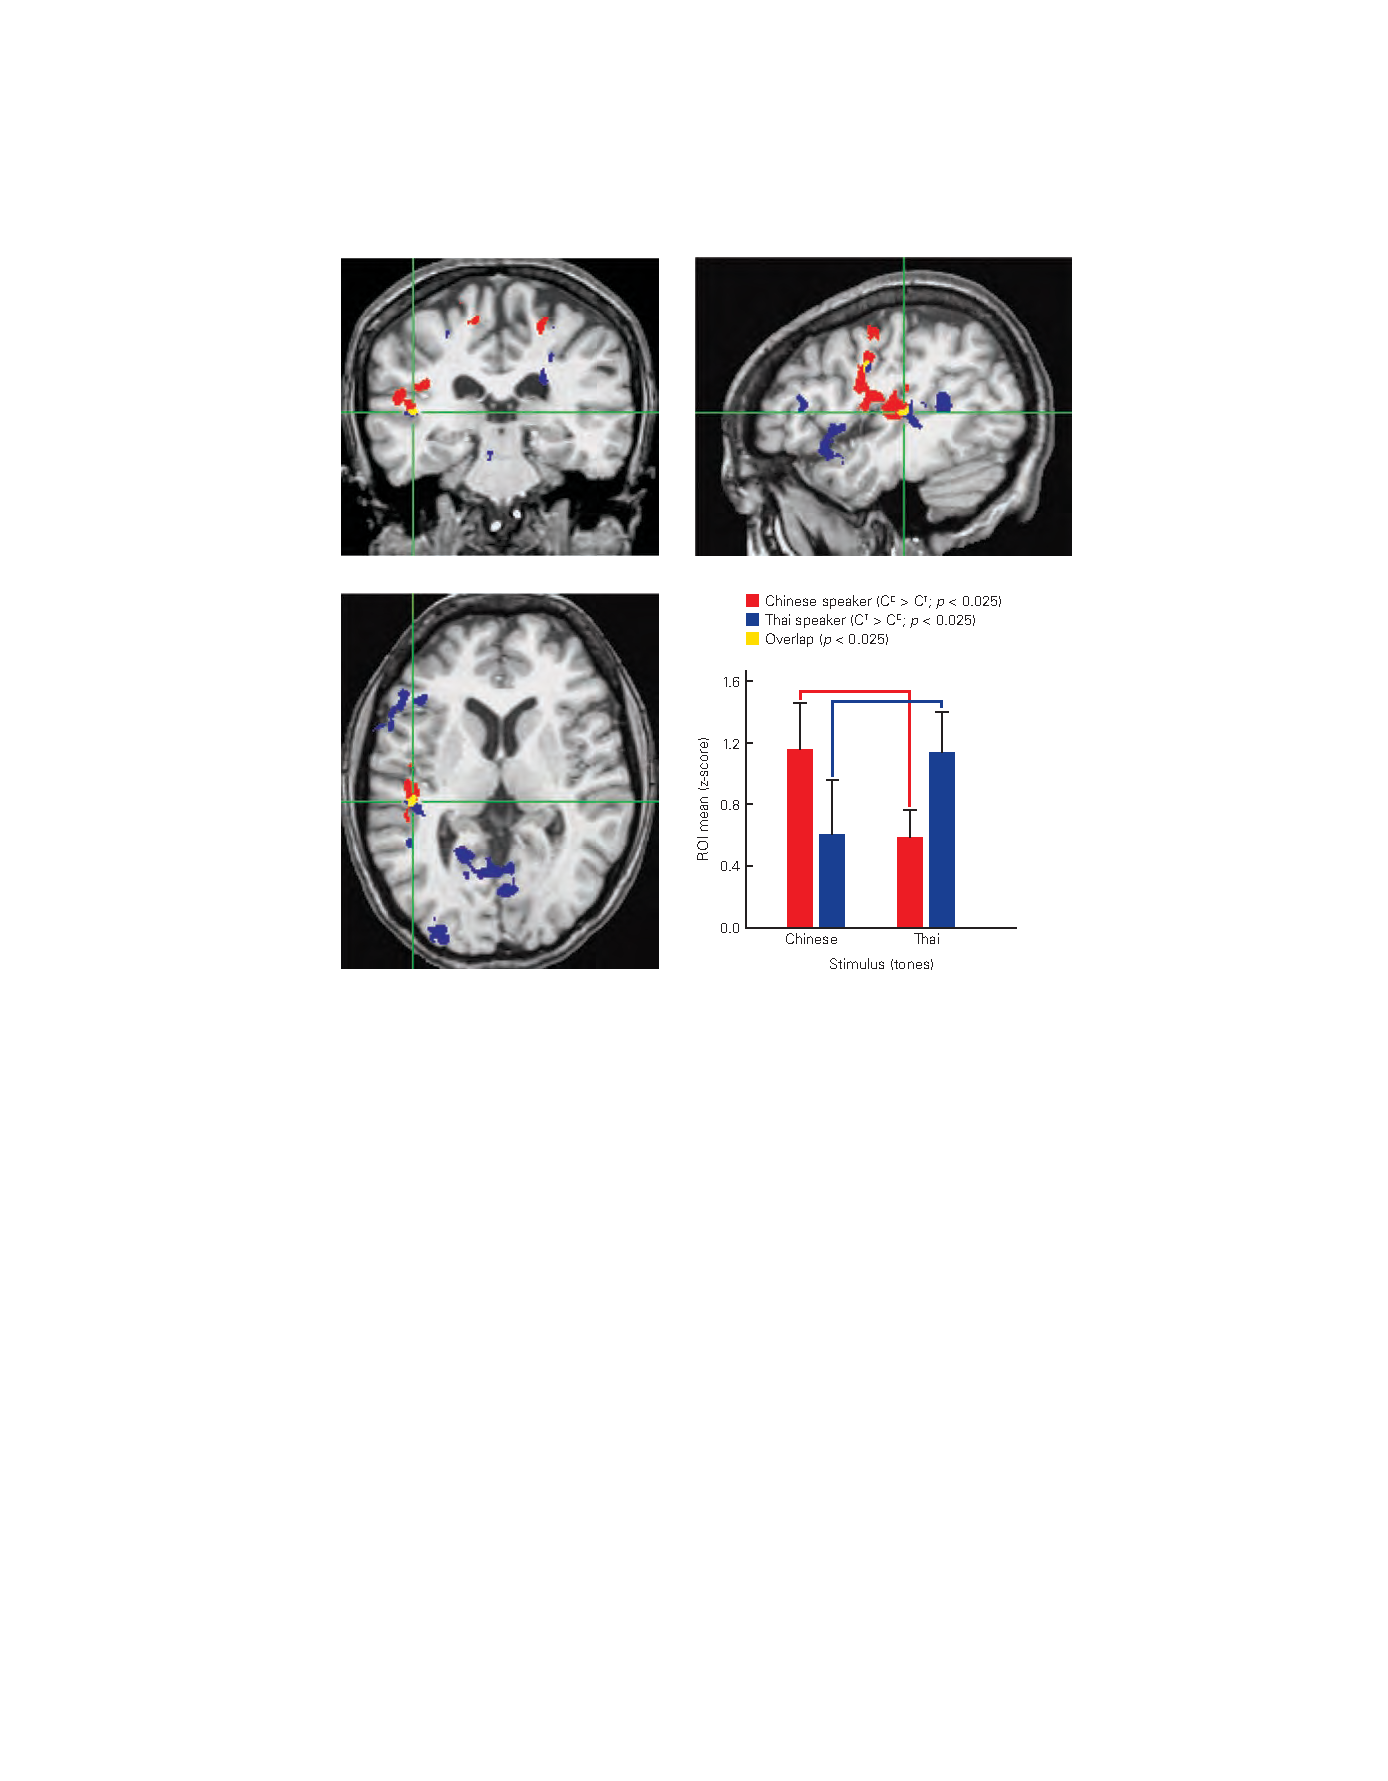
\includegraphics[width=0.88\linewidth]{chap55/fig_55_5}
	\caption{功能性磁共振成像显示的汉语和泰语词汇声调的大脑激活。
		语言刺激由汉语音节叠加泰语声调($ C^T $)或汉语声调($ C^C $)组成。
		以中文为母语的人和以泰语为母语的人在听母语时都表现出\textit{左半球}优势。
		在讲中文的人中,左半球对中文声调的激活更强,而在讲泰语的人中,对泰语声调的激活更强。
		两组的重叠发生在左侧颞叶平面和腹侧中央前回。
		在左侧的颞平面(绿色十字线)中,在音调处理和语言体验(条形图)之间发现了双重分离。
		\textit{右半球}没有表现出这些影响\cite{xu2006activation}。
		(左上角,冠状切面;右上角,矢状切面;左下角,轴向切面。)}
	\label{fig:55_5}
\end{figure}


\section{失语症的研究为语言处理提供了见解}

根据最近的估计,美国每年有超过 79 万 5 千 例中风。
失语症发生在 21\% 至 38\% 的急性中风中,并增加了死亡率和发病率的可能性。
在过去十年中,患有失语症的人数每年增长超过 10 万人。
布罗卡失语、韦尼克失语和传导性失语构成了临床失语综合症的三种经典模型。
\textit{希科克}和\textit{波佩尔}在双流模型的背景下描述了这些亚型中的每一个。
因此,布罗卡氏失语症和传导性失语症是由于与语言处理背侧流受损相关的感觉运动整合问题,而韦尼克氏失语症、词性耳聋和经皮层感觉性失语症是由腹侧流受损引起的。



\subsection{布洛卡失语症是由左额叶的大损伤引起的}

布罗卡失语症是一种言语产生障碍,包括由背侧流损伤引起的语法处理障碍。
当我们说话时,我们依赖大脑中存储的听觉模式。
当出现咖啡时,为杯子命名需要患者将存储的与“杯子”一词相关的感觉模式与击中该听觉目标所需的运动计划联系起来。
对于布罗卡失语症,流利言语产生所必需的感觉运动整合受损。
因此,说话吃力而缓慢,发音受损,并且缺乏正常说话的旋律语调(表~\ref{tab:55_2})。
然而,患者有时在口头交流方面取得了相当大的成功,因为他们对某些类型的单词,尤其是名词的选择通常是正确的。
相比之下,动词和语法词(如介词和连词)选择不当或可能完全缺失。
布罗卡失语症的另一个主要迹象是重复复杂句子的能力存在缺陷。


\begin{table}[htbp]
	\caption{原发性失语症患者自发言语产生和重复的例子} \label{tab:55_2} \centering
	\begin{tabular}{lll}
		\toprule
		失语症的类型 & 自然口语 & 重复 \\
		\midrule
		 & \makecell[l]{刺激(西方失语症炮台野餐图片):\\你在这张图片中看到了什么?} & 刺激:“糕点师很高兴。” \\
		布洛卡 & \makecell[l]{“O, yea. Det’s a boy an’ a \\girl . . . an’ . . . a . . . \\car . . . house . . . light po’ \\ (pole). Dog an’ a . . . boat.\\ ‘N det’s a . . . mm . . . \\a coffee, an’ reading. \\ Det’s a mm . . . a . . . \\det’s a boy . . . fishin’.” \\(所用时间:1 分 30 秒)} & “Elated.” \\
		韦尼克 & \makecell[l]{“Ah, yes, it’s, ah . . . several things. \\It’s a girl . . . uncurl . . . on a boat. \\ A dog . . . ‘S is another dog . . . \\Uh-oh . . . long’s . . . on a boat. \\The lady, it’s a \\ young lady. An’ a man a They were \\eatin’. ‘S be place there. \\This . . . a tree! A \\boat. No, this is a . . . It’s a\\ house. Over in here . . . a cake. \\An’ it’s, it’s a lot of \\water. Ah, all right. I think I mentioned\\ about that boat. I noticed a boat being \\ there. I did mention that before. . . . \\Several things down, different things \\	down . . . a bat . . . a cake . . . \\you have a . . .”  (所用时间:1 分 20 秒)} & “/I/ . . . no . . . In a fog.” \\
		传导 & \makecell[l]{“Kay. I see a guy readin’ a book. \\See a women /ka . . . \\he . . . /pourin’ drink \\ or something. An’ they’re sittin’ \\under a tree. An’ there’s a . . . \\car behind that \\ an’ then there’s a house behind th’ car. \\An’ on the other side, the guy’s flyn’ \\ a /fait . . . fait/(kite). See a dog there \\an’ a guy down on the bank. See a flag \\ blowin’ in the wind. Bunch of /hi . . . \\a . . . /trees in behind. An a sailboat on \\ th’ river, river . . . lake. ‘N guess that’s \\about all. . . . ‘Basket there.” \\(所用时间:1 分 5 秒)} & \makecell{“The baker was . . . What \\ was that last word?” \\ (“Let me repeat it: The \\ pastry cook was elated.”) \\ 	“The baker-er was / \\ vaskerin/ . . . uh . . .”} \\
		全面 & 嘟哝着说 & (无响应) \\
		\bottomrule
	\end{tabular}
\end{table}


由于大多数布罗卡失语症患者给人的印象是能听懂对话,所以最初认为这种情况只是语言表达障碍。
但是布罗卡失语症患者很难理解其含义主要取决于语法的句子。
布罗卡失语症可以理解女孩吃的苹果是绿色的,但难以理解男孩追的女孩是高个子。
这是因为他们无需借助语法规则就能理解第一句话:女孩吃苹果,但苹果不吃女孩;
苹果可以是绿色的,但女孩不能。
然而,他们对第二句话有困难,因为女孩和男孩都可以很高,并且可以追逐另一个。
要理解第二句话,就要分析它的语法结构,这是布罗卡失语症难以做到的。


布罗卡失语症是由于布罗卡区(左侧额下回)受损所致; 周围的额叶区域; 底层的白质、脑岛和基底神经节; 和前颞上回的一小部分(图 \ref{fig:55_6})。
脑岛的一小部分,一个深埋在大脑半球内部的皮层岛,也可以包括在布罗卡失语症的神经相关物中。
布罗卡失语症患者通常在感知语音或识别自己的错误方面没有困难,并且在想出单词方面也没有困难。
当损伤仅限于布罗卡区或其下方的白质时,结果就是布罗卡区失语症,这是一种较温和的真布罗卡区失语症,许多患者能够从中恢复。


\begin{figure}[htbp]
	\centering
	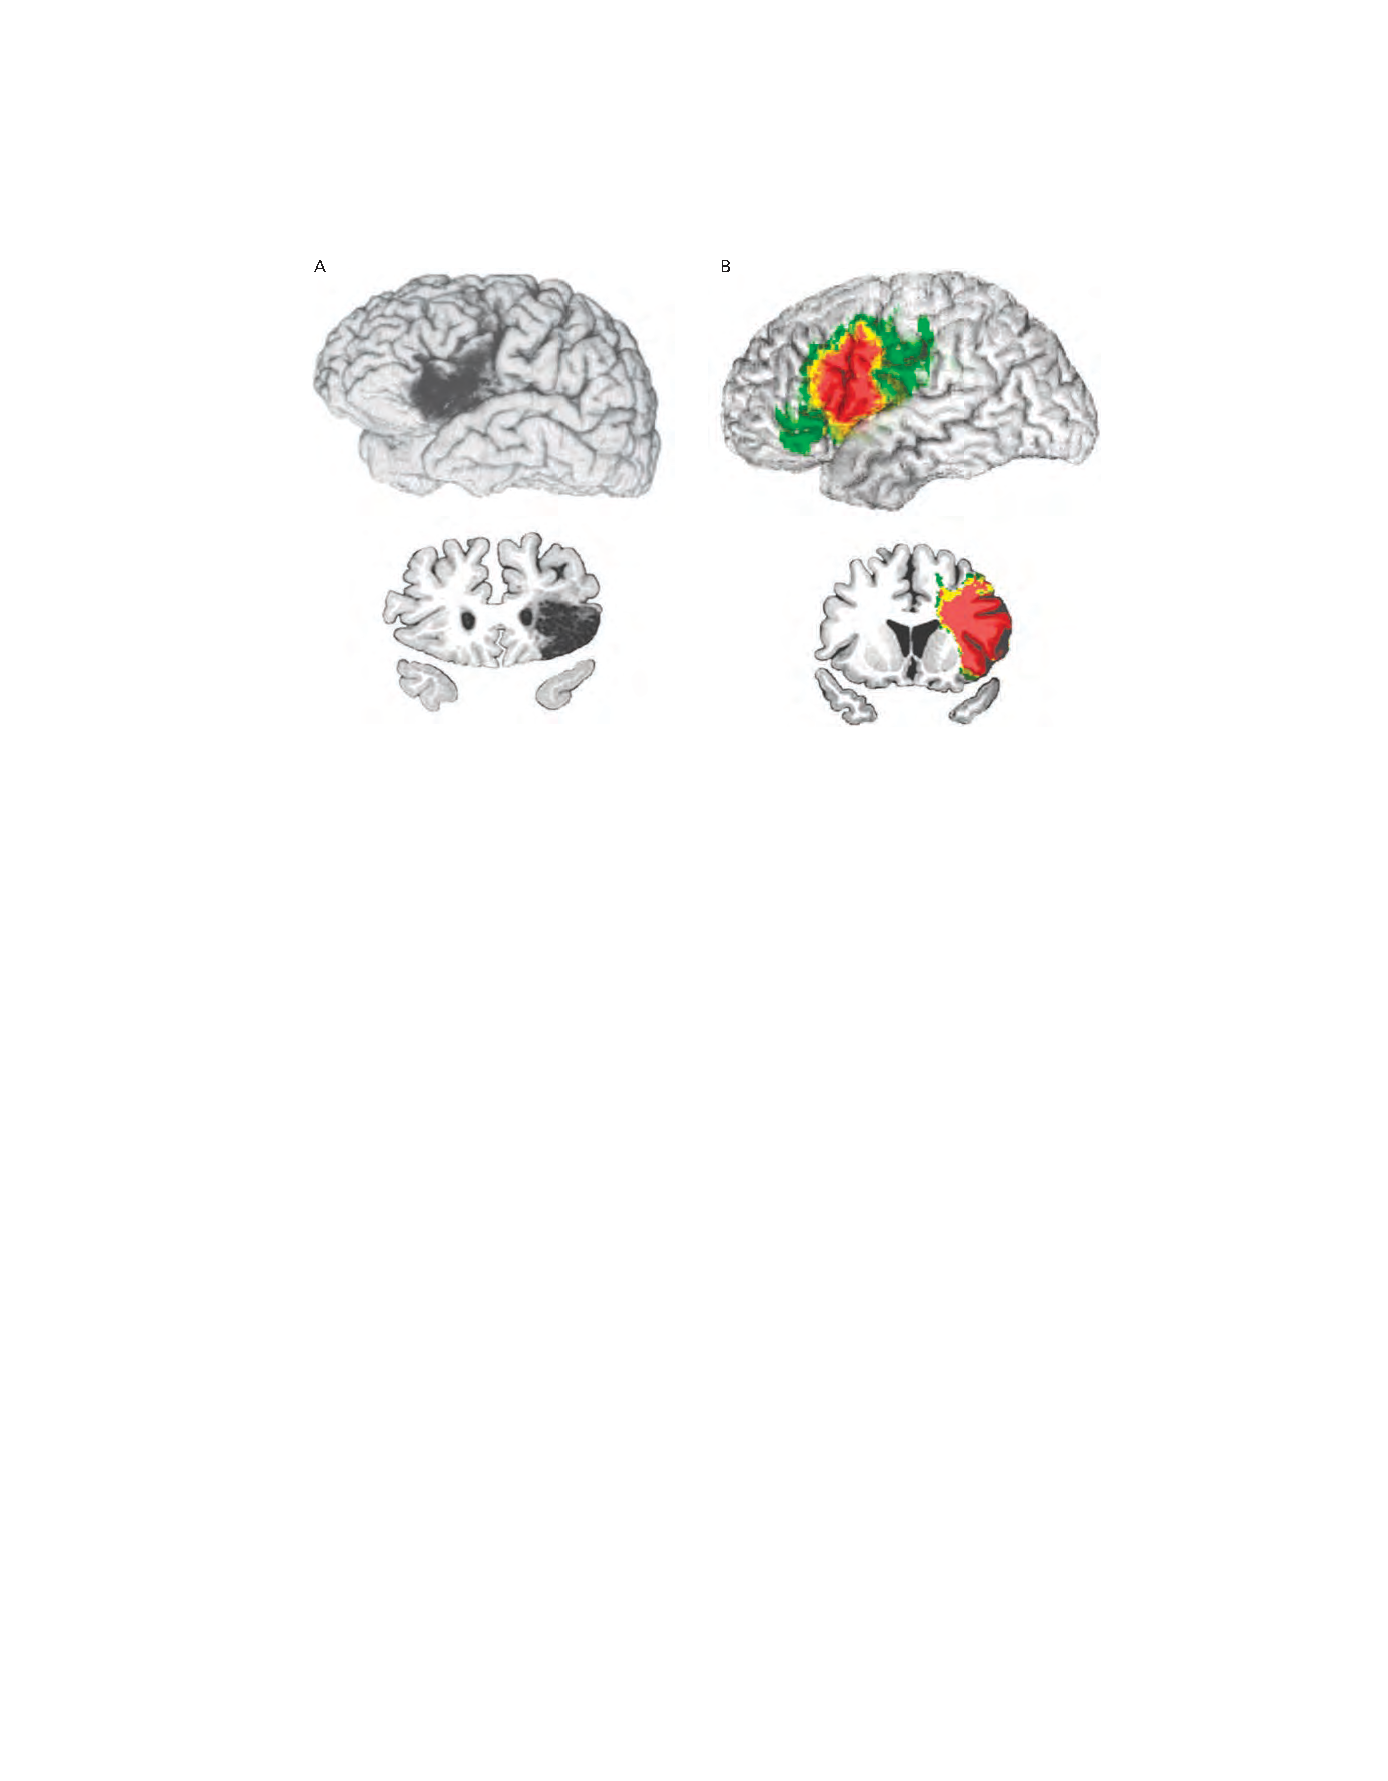
\includegraphics[width=0.8\linewidth]{chap55/fig_55_6}
	\caption{布罗卡失语症的病变部位。
		\textbf{A.} 上图:布罗卡失语症患者左侧额盖(深灰色)病变(梗死)的三维\textit{磁共振成像}重建图。
		底部:穿过受损区域的同一大脑的冠状\textit{磁共振成像}切片。
		\textbf{B.} 上图:13 名布罗卡失语症患者病灶的三维\textit{磁共振成像}重叠(红色表示 5 名或更多患者的病灶共享相同的像素)。
		底部:通过受损区域的同一复合脑图像的冠状\textit{磁共振成像}切片。}
	\label{fig:55_6}
\end{figure}



\subsection{韦尼克的失语症是由于左侧后颞叶结构受损所致}

韦尼克失语症患者难以理解他人所说的句子,大脑中负责语法、注意力和词义的区域会受到损害。
韦尼克失语症可能是由于腹侧流不同水平的损伤引起的,听觉信息与单词知识相关联。
它通常是由左侧听觉联合皮层后部损伤引起的,但在严重的情况下,会涉及颞中回和白质(图~\ref{fig:55_7})。


\begin{figure}[htbp]
	\centering
	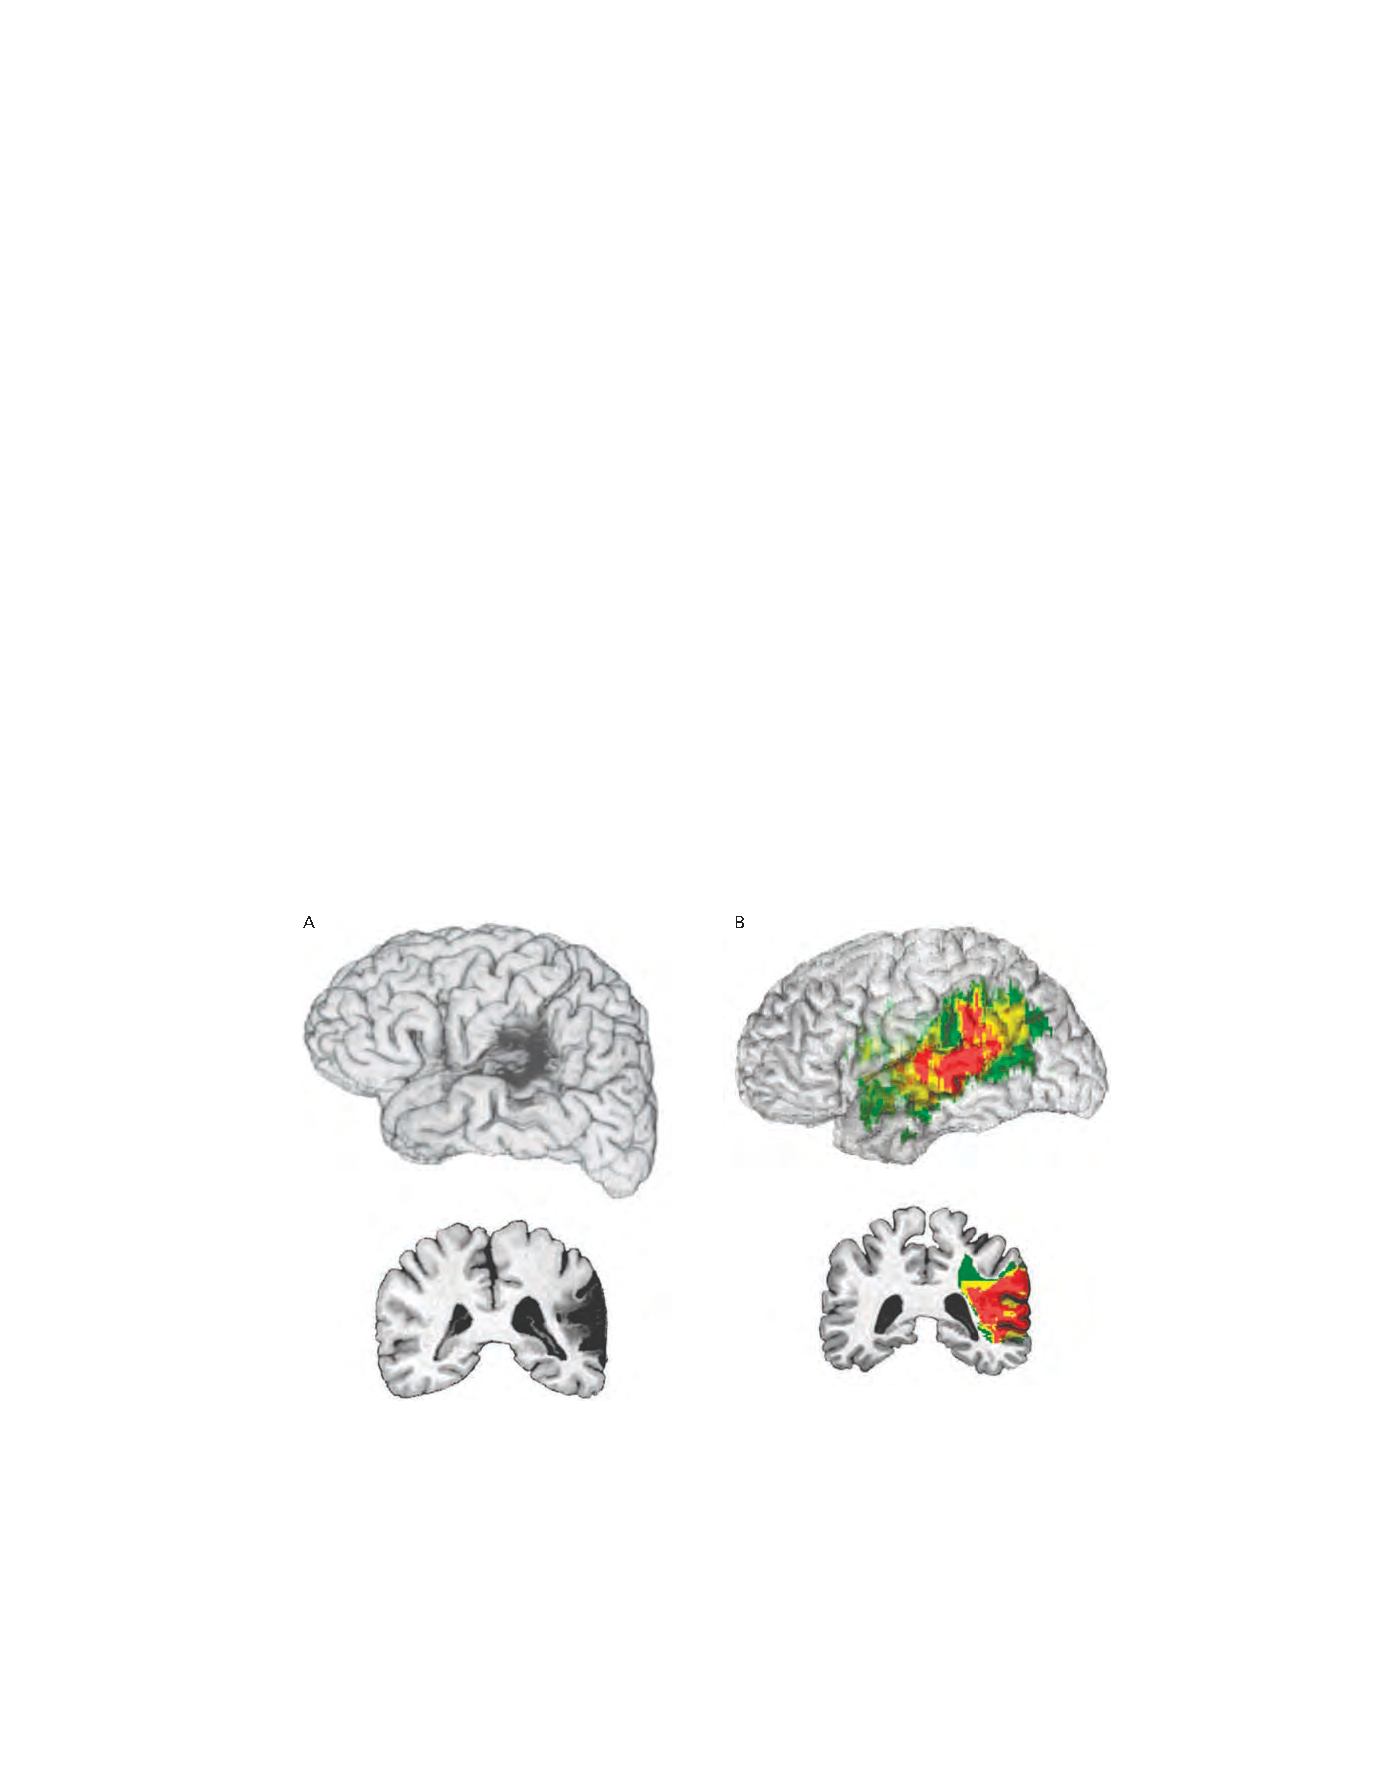
\includegraphics[width=0.75\linewidth]{chap55/fig_55_7}
	\caption{韦尼克失语症的病变部位。
		\textbf{A.} 上图:患者左后颞叶皮层(深灰色)病变(梗塞)的三维\textit{核磁共振成像}重建 与韦尼克失语症。
		底部:通过受损区域的同一大脑的冠状\textit{核磁共振成像}切片。
		\textbf{B.} 顶部:使用 MAP-3 技术获得的 13 名韦尼克失语症患者病灶的三维\textit{核磁共振成像}重叠(红色表示五个或更多病灶共享相同的像素)。
		底部:通过受损区域的同一复合脑图像的冠状\textit{核磁共振成像}切片。}
	\label{fig:55_7}
\end{figure}


韦尼克失语症患者能够以正常的语速说话,听起来毫不费力,旋律优美,与布罗卡失语症患者完全不同。
但语音也可能难以理解,因为韦尼克失语症经常改变单个声音和声音群的顺序。
这些错误称为音位错语(错语是用错误的音素代替正确的音素)。
即使正常发出单个声音,韦尼克失语症也很难选择准确表示其预期含义的词(称为语言或语义失语症)。
例如,当患者指的是总统时,他们可能会说首领。


\subsection{传导性失语症是由后语言区的一部分受损引起的}

传导性失语症与布罗卡氏失语症一样,被认为涉及背侧流。
与其他两种主要失语症相比,言语产生和听觉理解受到的损害较小,但患者不能逐字重复句子,不能有效地组合音素(因此产生许多音素性错语),并且不能轻易命名图片和物体(表~\ref{tab:55_2})。


传导性失语是由左侧颞上回和下顶叶损伤引起的。
损伤可延伸至左侧初级听觉皮层、脑岛和下方的白质。
位于听觉和运动区域网络中间的侧裂顶叶颞区的大损伤与损伤发生在背侧流的观点一致。
左半球听觉区域的损伤通常会导致言语产生缺陷,支持感官系统参与言语产生的观点。
这种损伤会中断连接单词听觉表征和用于产生它们的运动动作的接口。
这种损伤会损害白质(背侧流)并影响连接颞叶、顶叶、岛叶和额叶皮层区域的前馈和反馈投射。



\subsection{完全性失语症源于多个语言中心的广泛受损}

全面性失语症患者几乎完全无法理解语言或组织和重复句子,因此结合了布罗卡失语症、韦尼克失语症和传导性失语症的特征。
讲话最多减少到几句话。
可能会重复使用同一个词,无论是否恰当,以徒劳地试图传达一个想法。
然而,可以保留非故意的(“自动的”)语音。
这包括常用的咒骂语(使用得当并且具有正常的音位、语音和屈折变化结构)、例行程序(例如计算或背诵一周中的日子)以及唱出以前学过的旋律及其歌词的能力。
听觉理解仅限于少数单词和惯用语。


经典的整体性失语症涉及对下额叶和顶叶皮层(如\textit{布洛卡}失语症所见)、听觉皮层和脑岛(如传导性失语症所见)以及后上颞叶皮层(如韦尼克失语症所见)的损害。
皮层下区域,例如基底神经节,也经常受到影响。
这种广泛的损伤通常是由大脑中动脉供应区域的中风引起的。
典型的全身性失语症伴有右侧面部无力和右肢瘫痪。



\subsection{布罗卡区和韦尼克区附近区域受损导致经皮层失语}

失语症不仅可以由大脑皮层的语言中心受损,还可以由连接这些组件与大脑其余部分的通路造成。
经皮层失语可以是运动性的或感觉性的。
经皮层运动性失语症患者说话不流利,但他们可以重复句子,甚至是很长的句子。
经皮层运动性失语症与左侧额叶背外侧区的损伤有关,该区域是布罗卡区前面和上方的一块联合皮层,尽管布罗卡区本身可能会受到实质性损伤。
左背外侧额叶皮层参与注意力的分配和高级执行能力的维持,包括单词的选择。


皮层运动性失语症也可能是由于左侧辅助运动区受损引起的,该区域位于额叶高处,直接位于初级运动皮层前方,并埋在两个半球之间。
对非失语症手术患者的该区域进行电刺激会导致患者不自主地发声或无法说话,功能性神经影像学研究表明它在言语产生过程中被激活。
因此,辅助运动区似乎有助于语言的启动,而背外侧额叶区域有助于持续控制语言,尤其是在任务困难时。


经皮层感觉性失语症患者言语流畅、理解能力受损,并且在命名事物时遇到很大困难。
这些患者在语义检索方面存在缺陷,句法和语音能力没有明显中断。


经皮层运动和感觉性失语是由弓状束和背侧束的损伤引起的。
因此,在行为和解剖学上,经皮层失语症是传导性失语症的补充。
经皮层感觉性失语症似乎是由腹侧流损伤引起的,影响了颞叶、顶叶和枕叶交界处的部分区域,这些区域将大脑外侧语言区与负责词义的大脑部分连接起来。



\subsection{不太常见的失语症涉及对语言重要的其他大脑区域}

大脑皮层和皮层下结构中其他几个与语言相关的区域,例如前颞叶和下颞皮层,最近才与语言相关联。
左颞叶皮层的损伤会导致严重而纯粹的命名缺陷:单词检索的障碍,但没有任何伴随的语法、音素或语音困难。


当损伤局限于左侧颞极时,患者难以回忆起独特的地方和人物的名称,但不能回忆起常见事物的名称。
当病变累及颞中部时,患者很难回忆起独特的和常用的名字。
最后,左后下颞区的损伤导致无法回忆起特定类型物品(工具和用具)的单词,但无法回忆起自然或独特事物的单词。
对动作或空间关系的词语的回忆不会受到影响(图~\ref{fig:55_8})。


\begin{figure}[htbp]
	\centering
	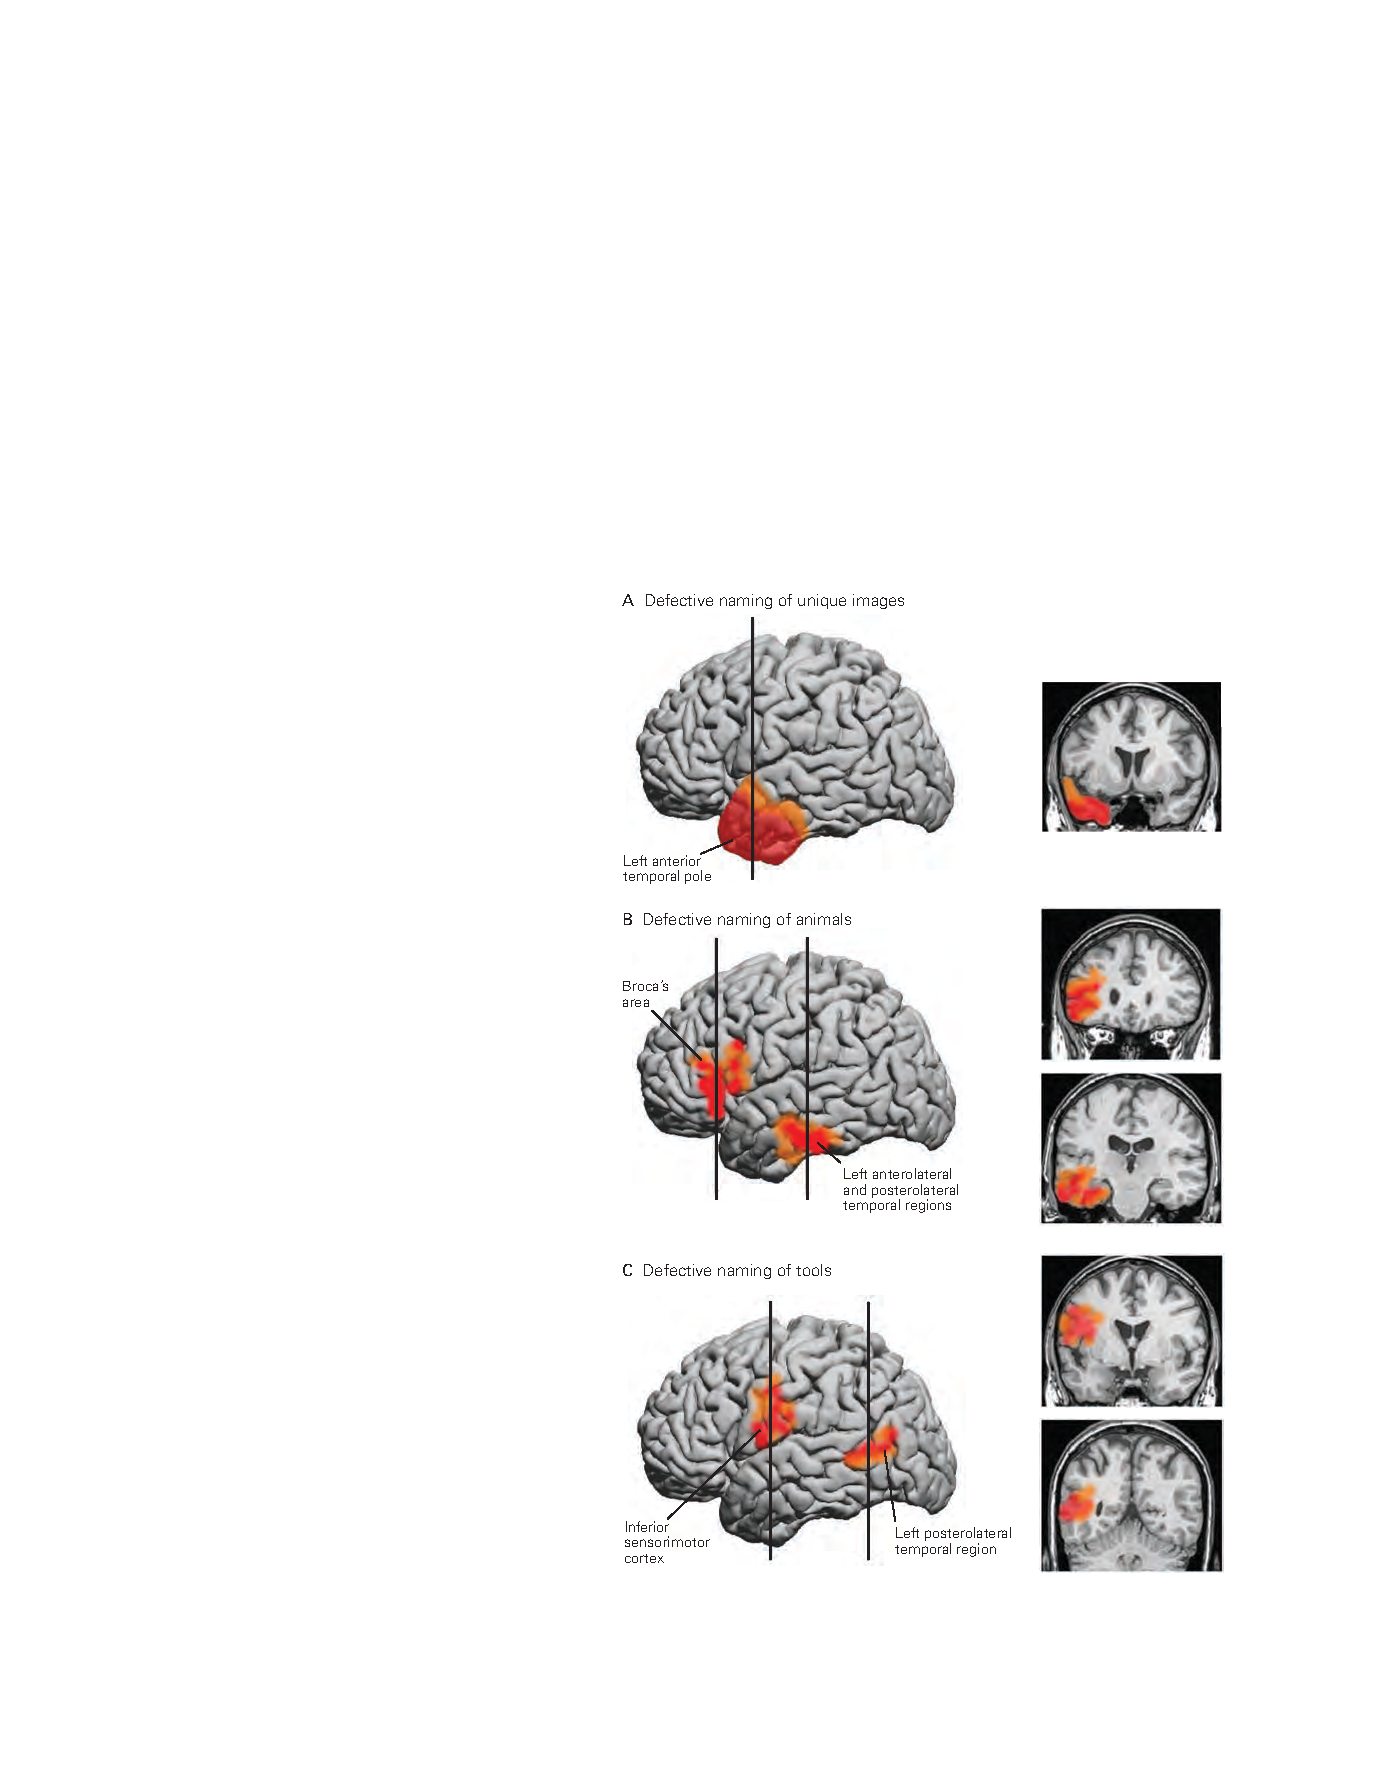
\includegraphics[width=0.79\linewidth]{chap55/fig_55_8}
	\caption{大脑中除布罗卡区和韦尼克区以外的区域都涉及语言处理。
		\textit{功能性核磁共振成像}用于研究具有选定脑部病变的患者。
		\textbf{A.} 与独特图像(例如人脸)命名受损相关的病变最大重叠区域是左前颞极。
		\textbf{B.} 与非独特动物命名受损相关的病变最大重叠部位是左侧前外侧和后外侧颞区以及布罗卡区。
		\textbf{C.} 与工具命名缺陷相关的病变最大重叠部位是左侧感觉运动皮层和左侧后外侧颞叶皮层。}
	\label{fig:55_8}
\end{figure}


左颞叶皮层包含神经系统,这些神经系统掌握着检索表示各种事物类别(“工具”、“餐具”)的词的关键,但不包含表示动作的词(“步行”、“骑自行车”)。
这些发现不仅来自对中风、头部受伤、疱疹性脑炎和阿尔茨海默病等退行性过程引起的脑损伤患者的研究,还来自典型个体的功能成像研究以及对这些相同颞区的电刺激 手术过程中的皮层。


左半球近中表面的额叶皮层区域,包括辅助运动区和前扣带回区,在言语的发起和延续中起着重要作用。
这些区域的损伤会影响运动的启动(运动不能)并导致缄默症,即完全无法说话。
在失语症患者中,完全没有言语是罕见的,并且只在病情的早期阶段才会出现。
运动不能症和缄默症患者无法通过语言、手势或面部表情进行交流,因为交流的动力受损,而不是因为表达的神经机制受损,如失语症。


左侧皮层下灰核的损伤会损害言语和理解的语法处理。
基底神经节与额叶和顶叶皮层紧密相连,可能在将词素组合成单词和将单词组合成句子方面发挥作用,就像它们将复杂运动的组成部分组合成流畅的动作一样。



\section{亮点}

1. 语言有很多层次,每个层次都必须在童年时期掌握,用于改变单词含义的基本语音单元(元音和辅音)、单词本身、改变时态和复数的词尾(语素),以及允许将单词串在一起以创建有意义的句子的语法规则。
到 3 岁时,无论学习何种语言,年幼的孩子都已经掌握了所有级别,并且可以与成人进行对话。
目前还没有人工智能机器可以复制这一壮举。 


2. 1岁以下儿童掌握语言的学习策略令人惊讶。
语言学习从婴儿时期开始(1)利用语音的统计特性(声音的分布频率模式来检测相关的语音单元和相邻音节之间的过渡概率来检测可能的单词),以及(2)利用语言出现的社会背景 跟随成人指代物体和动作时的眼球运动来学习词-物体和词-动作的对应关系。
在早期,自然语言学习需要社会背景和社会互动。
斯金纳操作性条件反射或乔姆斯基基于经验的先天表征和选择并不能很好地描述婴儿的策略。
相反,在社会环境中运作的强大的内隐学习机制使婴儿从生命的最初几个月开始就向前发展。


3.婴儿的言语产生和言语感知能力在出生时是“通用的”。
在语音感知方面,婴儿在 6 个月大之前能够辨别所有语言中用于区分单词的所有声音。
到 12 个月大时,对母语发音的辨别力急剧增加,而对外语发音的辨别力则下降了。
生产最初也是通用的,并在第一年年底成为特定语言。
到 3 岁时,婴儿知道 1 千个单词。
复杂句子中语法结构的掌握一直持续到 10 岁。
未来的工作将通过将现在存在的详细行为里程碑与功能和结构大脑测量联系起来来推进该领域,以显示大脑的语言网络是如何根据语言经验形成的。 


4. 基于过去十年中功能神经成像和结构脑成像的进步,出现了一种新的“双流”语言模型。
新模型与视觉系统的双流模型有相似之处。
语言的双流模型超越了经典的韦尼克-格施温德模型,表明许多大脑区域和连接它们的神经通路支持声音到意义(腹侧)和声音到发音(背侧)通路。
随着更多研究显示行为和大脑测量之间的关系,模型的改进将继续进行。
未来的研究将整合大脑的结构和功能测量、遗传测量以及语言处理和学习的行为评估,包括成年期的第二语言学习。


5. 对婴儿大脑的研究表明,到 3 至 6 个月大时,大脑结构和通路已经非常发达。
结构性\textit{弥散张量成像}揭示了出生时完全形成的腹侧通路和连接听觉区与运动前区而非出生时布罗卡区的背侧通路。
\textit{脑电图}和\textit{脑磁图}大脑成像研究反映了 6 到 12 个月大时语音感知的转变,这是声音学习的“关键时期”。
这一时期的\textit{脑磁图}脑部扫描揭示了当婴儿听到语音时听觉和运动中枢的共同激活,并显示感觉和运动大脑区域的变化是经验的函数。
数据表明,第一年的背侧通路已经充分形成,可以支持这一时期的感觉-运动连接和模仿学习。


6. 半球专业化通常随着年龄和语言经验的增加而增加,区域和路径的初步代表是双侧代表的,并且随着语言经验的出现而出现优势。
然而,对于不同水平的语言,侧化程度存在差异。
调节语音的听觉运动表征的背侧流比调节单词的听觉概念表征的腹侧流更偏左。


7. 经典的失语症(布罗卡失语症、韦尼克失语症和传导性失语症)在双流语言模型的背景下得到了很好的描述。
布罗卡失语症强调无法产生言语但相对较好的言语理解,被视为背侧流缺陷,而韦尼克失语症强调言语理解缺陷,被视为腹侧流缺陷。
传导性失语症与布罗卡氏症一样,被认为是由背流缺陷引起的,其损害包括听觉和运动区域。
未来对失语症的研究将受益于对功能和结构损伤的额外研究,这些研究可以与详细的行为协议相结合。 


8. 未来的研究将允许对人类和非人类大脑进行详细比较,以揭示人类独有的结构和通路,这些结构和通路支持语言。
未来的工作还将关注人类语言结构在多大程度上被语音选择性地激活,而不是其他复杂的听觉声音,以及成人水平的选择性是否在发育早期存在。 


9. 人类语言代表了人类认知成就的一个独特方面。
了解几乎所有儿童都具备这种认知能力的大脑系统,尤其是发现识别有语言发育障碍风险的儿童的生物标志物,将推动脑科学的发展并造福于社会。
现在,行为研究使我们能够将早期语言经验与儿童入学时的高级语言发展之间的联系联系起来。
这可能会导致语言干预,从而改善所有儿童的结果。



